\chapter{Evolutionary Algorithms}\label{ch:ea}
Finally, we turn our eyes to some of the coolest sounding AI techniques: \textit{Evolutionary} and \textit{Genetic Algorithms}. In the previous (e.g., see Chapter \ref{ch:nn}), we have already seen that AI sometimes tries to mimic elements of real life (like our brains) to solve issues in Computer Science. Evolutionary algorithms is similar in that sense as the ideas behind it are inspired by biological evolution (see Aside \ref{as:evol}).

Evolutionary algorithms, and even wider, evolutionary computing, are a collection of optimisation algorithms, including\footnote{These following techniques largely differ in gene encoding and implementation details, but are considered a part of the same set of evolution inspired optimisation algorithms.}:
\begin{itemize}
\item\textbf{Genetic algorithm} (GA): the most popular type of EA, which seeks the solution of a problem in the form of strings of numbers, by applying operators such as recombination and mutations. Often used for optimisation problems.
\item\textbf{Genetic programming} (GP): a specific implementation of GA from the field of AI that creates optimised forms of computer programs. Given a number of (basic) program elements, the algorithm tries to combine these such that a suitable (well-performing) program is created for a known problem.
\item\textbf{Evolutionary programming}: similar to GP, but the structure of the program is fixed and its numerical parameters are allowed to evolve.
\item\textbf{Gene expression programming}: like GP, GEP evolves computer programs but it explores a genotype-phenotype system, where computer programs of different sizes are encoded in linear chromosomes of fixed length.
\item\textbf{Evolution strategy}: algorithm that works with vectors of real numbers as representations of solutions and typically uses self-adaptive mutation rates.
\item\textbf{Neuro-evolution}: similar to GP but the genomes represent artificial neural networks by describing structure and connection weights. 
\end{itemize}

In relation to the previous material of this course, it should not surprise you that we are trying to achieve neuro-evolution; that is, create an optimisation algorithm that can determine the best structure and weights for our neural networks. Before we get to the evolution of neural networks (see Section \ref{sec:neuroevolution}), we first have to explain what genetic algorithms are (see Section \ref{sec:ga}) and how they function.

\section{Genetic algorithms}\label{sec:ga}
Genetic algorithms are a metaheuristic from the field of computer science (more specifically, operations research). Being inspired by the concepts of biological evolution, they belong to the larger class of \textit{evolutionary algorithms}. While genetic and evolutionary algorithms are considered a part of computer science, the study of the use of evolution inspired algorithms, broadly called \textit{evolutionary computing}, is in fact a sub-field of Artificial Intelligence.

A \textit{metaheuristic} is a high-level procedure designed to find, generate, or select a heuristic\footnote{A heuristic is a search method that uses knowledge of the problem to avoid having to search the entire solution space. While this provides efficiency (solutions can be found faster), the disadvantage is that it is not guaranteed that the (overall) best solution will be found.} (partial search algorithm) that may provide a sufficiently good solution to an optimisation problem, especially with incomplete or imperfect information or limited computation capacity. Metaheuristics sample a set of solutions which is too large to be completely sampled; that is, they exploratively search a solution space without fully searching through that space to find a good enough solution to the problem. Compared to optimisation algorithms and iterative methods (e.g., binary search), metaheuristics do not guarantee that a globally optimal solution can be found.

Evolutionary algorithms (and therefore also genetic algorithms) use mechanisms inspired by evolution, such as \textit{reproduction}, \textit{mutation}, \textit{recombination}, and \textit{selection} to solve global optimisation or search problems.

\begin{aside}[Principles of evolution: \textit{On the Origin of Species}]~\label{as:evol}\\[2.5pt]
\begin{minipage}{0.7\textwidth}
In the mid-19th century, Charles Darwin formulated the scientific theory of evolution by natural selection, published in his book \textit{On the Origin of Species} \citeyearpar{darwin}. Evolution by natural selection is a process demonstrated by the observation that more offspring are produced than can possibly survive, along with three facts about populations:
\begin{enumerate}
\item traits vary among individuals with respect to morphology, physiology, and behaviour (phenotypic variation);
\item different traits confer different rates of survival and reproduction (differential fitness); and
\item traits can be passed from generation to generation (heritability of fitness).
\end{enumerate}
\end{minipage}
\hfill
\begin{minipage}{0.25\textwidth}
\includegraphics[width=\textwidth]{originOfSpecies}
\end{minipage}\\[2.5pt]
Thus, in successive generations members of a population are replaced by progeny of parents better adapted to survive and reproduce in the biophysical environment in which natural selection takes place.
\end{aside}

While not truly similar to natural selection as the goal of the selection is often predetermined in evolutionary algorithms, they adhere to the same principles of evolution: survival of traits is pertained by the implication of that trait on the overall fitness (that is, characteristics that make a (sub-)population perform better, survive longer), and important traits are passed from generation to generation (that is, children look like a combination of their parents, inheriting traits from both of them).

In principle, evolutionary algorithms function in this rudimentary manner:
\begin{enumerate}
\item Generation of an initial population of individuals (often at random);
\item Evaluation of the fitness of each individual in that population;
\item Repetition of the following re-generational steps until termination (or until a pre-defined maximal number of generations):
\begin{enumerate}
\item Select the best-fit individuals for reproduction;
\item Breed new individuals through crossover and mutation operations to give birth to offspring.
\item Evaluate the individual fitness of new individuals.
\item Replace least-fit population with new individuals.
\end{enumerate}
\end{enumerate}

\begin{aside}[What's in a name]~\\
The use of Evolutionary principles for automated problem solving originated in the 1950s. It was not until the 1960s that three distinct interpretations of this idea started to be developed in three different places.

\textit{Evolutionary programming} was introduced by Lawrence J. Fogel in the US, while John Henry Holland called his method a \textit{genetic algorithm}. In Germany Ingo Rechenberg and Hans-Paul Schwefel introduced \textit{evolution strategies}. These areas developed separately for about 15 years. From the early nineties on they are unified as different representatives (``dialects'') of one technology, called \textit{evolutionary computing}. Also in the early nineties, a fourth stream following the general ideas had emerged – \textit{genetic programming}. Since the 1990s, nature-inspired algorithms are becoming an increasingly significant part of evolutionary computation.
\end{aside}

\begin{figure}[h!]
\centering
\includegraphics[width=0.4\textwidth]{evolvedAntenna}
\caption{2006 NASA ST5 spacecraft antenna, found by an evolutionary computer design program to create the radiation pattern.}\label{fig:antenna}
\end{figure}

In the following we look at each of these steps in turn (with a running example) to show how genetic algorithms are used.

\begin{aside}[Genetic programming]~\\
Genetic programming (GP) is an AI technique whereby computer programs are encoded as a set of genes that are then modified (evolved) using an evolutionary algorithm (often a genetic algorithm). The results are computer programs able to perform well in a predefined task.\\[0.5pt]
\begin{minipage}{0.5\textwidth}
The methods used to encode a computer program in an artificial chromosome and to evaluate its fitness with respect to the predefined task differ between techniques and is still a subject of research. As an example, a computer program could be represented as a tree structure (favouring functional programming languages), which can be evaluated in a recursive way, making mathematical expressions easy to evolve and evaluate.
\end{minipage}\hfill
\begin{minipage}{0.45\textwidth}
\centering
\includegraphics[width=0.85\textwidth]{geneticProgramming}
\end{minipage}\\[2.5pt]
The genetic algorithm is then employed to optimise the structure and position of elements within the tree, with the aim of creating the fittest program to solve the problem.
\footnote{Picture by Wikipedia.}
\end{aside}

\subsection{Optimisation}\label{sec:fitness}
In mathematics and computer science, optimisation is the selection of a best element (with regard to some criterion) from some set of available alternatives. In the simplest case, an optimisation problem consists of maximising or minimising a real function by systematically choosing input values from within an allowed set and computing the value of the function. More generally, optimisation includes finding "best available" values of some objective function given a defined domain (or input), including a variety of different types of objective functions and different types of domains.

The purpose of an optimisation problem is to find a solution $s_{max}\in S$, that is find the maximal solution $s_{max}$ in a given solution space $S$. Because the solution space is often too large to search systematically (that is, select each solution individually and determine whether it is the best (so far)), heuristic searches are often applied. Genetic algorithms is one of these, but gradient descent, presented earlier in Section \ref{sec:gradient}, is another\footnote{Note that gradient descent is doing the exact opposite by trying to minimise the value of $s$; that is, find the lowest point $s_{min}$ in the solution space $S$. The principle is the same, however.}. A third optimisation technique, that is close to how genetic algorithms work, is (local) \textit{hill climbing}.

\begin{figure}[h!]
\centering
\includegraphics[width=0.5\textwidth]{fitnessLandscape}
\caption{A fitness landscape.}\label{fig:fitness}
\end{figure}

As solution spaces are often quite big, and as their shape is not uniform, it can be quite challenging to find a optimal value. Consider the solution space in Figure \ref{fig:fitness}, if the fitness function (that is, the function that determines the score of a specific point) was known on forehand, it would be easy to determine where the maximum value would be (at least, it would be for us, as we can try to determine where the peak of the figure is). Unfortunately, the exact shape of the fitness function is not so obvious\footnote{Not to mention that most fitness functions are not 2-dimensional in shape; it is very difficult to imagine a 20-dimension shape and determine where the optimal value is.}, and only local information is known (we only know whether the points next to us are higher or lower), it can be very difficult to find the absolute maximum. In principle, this is how local hill climbing works, however. Local hill climbing starts a some random point and tries (randomly) its neighbours to see if one of those has a higher fitness than itself.

\begin{algorithm}[Local hill climbing]~\\
\begin{itemize}
\item Generate (or select) a starting solution $s_0$ at random, initialise time $t=0$;
\item Repeat until convergence:
\begin{enumerate}
\item create $s_{new}$ by changing $s_t$ (take a step left, forward, right, backward);
\item if the fitness of $s_new$ is bigger than that of $s_t$, then $s_{t+1}=s_{new}$ (we take $s_{new}$ as are next `starting point');
\item else $s_{t+1} = s_t$ (that is, we go back to our previous best point);
\item $t=t+1$ (increase time).
\end{enumerate}
\end{itemize}
\end{algorithm}

The most important aspect of the local hill climbing algorithm is \textit{changing $s_t$}. If the steps taken are too small, progress will be very slow; but if the steps are too large, optimal values might be overstepped and never found.

\begin{figure}[h!]
\centering
\includegraphics[width=0.45\textwidth,trim={0 1.75cm 0 2cm},clip]{hillclimb1}
\hfill
\includegraphics[width=0.45\textwidth]{hillclimb2}
\caption{Hill climbing in 3D (left) and 2D (right).}\label{fig:hill}
\end{figure}

An important disadvantage of hill climbing is that the algorithm is prone to getting stuck in local optima (that is, a peak that is smaller than the optimal peak, but high enough that a step in either direction does not affect an immediate improvement). Consider for instance the red and green paths in the left-hand side of Figure \ref{fig:hill}; or the paths $A$ and $C$ in the right-hand side of Figure \ref{fig:hill}. It is therefore important to run the algorithm multiple times, with different starting points.

On an abstract level, genetic algorithms function in similar matter. By selecting the best traits in individuals, genetic algorithms try to only take the steps that are `uphill'. The biggest distinction between genetic algorithms and the hill climbing algorithm is, however, that genetic algorithms use many different starting points (thus trying to circumvent the local optima problem of hill climbing) and can, given correct parameter choices, escape local optima.


\subsection{Problem definition}
To use a genetic algorithm on a optimisation problem, we have to start with a representation of the problem and its solutions. Candidate solutions in a genetic algorithm are called \textit{individuals} or \textit{phenotypes}. The representation of an individual is called a \textit{genotype} (or genome), and there are many options to encode the individuals into a genotype. The encoding must be done in such a way that we can solve the problem. We have to consider the evaluation method used to determine the fitness of the individuals.

Genome representations can range from binary strings to arrays (or lists) of integer values or characters (or even program elements, in the case of genetic programming). An example of a binary representation is shown below:
\begin{center}
\begin{tikzpicture}
% \draw[step=1cm,gray,very thin] (0, 0) grid (9, 7);
\node[draw,minimum width=1cm, minimum height=1cm,fill=hured!20,anchor=south west,thick] at (0,0) {1};
\node[draw,minimum width=1cm, minimum height=1cm,fill=hured!20,anchor=south west,thick] at (1,0) {0};
\node[draw,minimum width=1cm, minimum height=1cm,fill=hured!20,anchor=south west,thick] at (2,0) {1};
\node[draw,minimum width=1cm, minimum height=1cm,fill=hured!20,anchor=south west,thick] at (3,0) {0};
\node[draw,minimum width=1cm, minimum height=1cm,fill=hured!20,anchor=south west,thick] at (4,0) {0};
\node[draw,minimum width=1cm, minimum height=1cm,fill=hured!20,anchor=south west,thick] at (5,0) {0};
\node[draw,minimum width=1cm, minimum height=1cm,fill=hured!20,anchor=south west,thick] at (6,0) {1};
\node[draw,minimum width=1cm, minimum height=1cm,fill=hured!20,anchor=south west,thick] at (7,0) {1};
\draw[decorate,decoration={brace,amplitude=10pt}] (0.5, 1.5) -- (7.5, 1.5);
\node at (4, 2.5) {chromosome};
\draw[decorate,decoration={brace,amplitude=5pt}] (5, -0.5) -- (4, -0.5);
\node at (4.5, -1.25) {gene};
\end{tikzpicture}
\end{center}

Given a representation of our genome, we have all the freedom to translate that into a phenotype. The genotype is the representation that is used in the search space (solution space); the phenotype is what is being evaluated.

\begin{center}
\begin{tikzpicture}
\node[draw,minimum width=1cm, minimum height=1cm,fill=hured!20,anchor=south west,thick] at (0,0) {1};
\node[draw,minimum width=1cm, minimum height=1cm,fill=hured!20,anchor=south west,thick] at (1,0) {0};
\node[draw,minimum width=1cm, minimum height=1cm,fill=hured!20,anchor=south west,thick] at (2,0) {1};
\node[draw,minimum width=1cm, minimum height=1cm,fill=hured!20,anchor=south west,thick] at (3,0) {0};
\node[draw,minimum width=1cm, minimum height=1cm,fill=hured!20,anchor=south west,thick] at (4,0) {0};
\node[draw,minimum width=1cm, minimum height=1cm,fill=hured!20,anchor=south west,thick] at (5,0) {0};
\node[draw,minimum width=1cm, minimum height=1cm,fill=hured!20,anchor=south west,thick] at (6,0) {1};
\node[draw,minimum width=1cm, minimum height=1cm,fill=hured!20,anchor=south west,thick] at (7,0) {1};
\node[anchor=north west] at (2.75, 2.5) {\large 8-bit genotype};
\node[anchor=north west] at (9, 2.5) {\large Phenotype:};
\node[anchor=north west] at (9, 2) {$\bullet$ integer};
\node[anchor=north west] at (9, 1.5) {$\bullet$ real number};
\node[anchor=north west] at (9, 1) {$\bullet$ schedule};
\node[anchor=north west] at (9, 0.5) {$\bullet$ \ldots};
\end{tikzpicture}
\end{center}
An example of an integer phenotype (given the genotype in the figure above) would be using the typical binary representation; $163$. If we would want to represent numbers between $2.5$ and $20.5$ (with maximal 256 values), the phenotype would be $2.5 + \frac{163}{256}(20.5-2.5)=13.9609$.

In some cases, for instance in parameter optimisation, we would rather base our genotype directly on real numbers. In this case we use a tuple (or list) of numbers, rather than a binary representation. For instance, to encode the order in which cities are visited in a Travelling Salesman Problem (TSP) can be done as follows\footnote{This encoding is ambiguous; it could either mean that the position in the genome determines the position in the route (i.e., city $3$ is visited first, then city $4$, etc.), or the position in the genome determines the city, and the number indicates the position in the route (i.e., city $5$ is visited first, then city $6$, etc.). Either encoding would work, as long as the fitness function is defined correctly.}:
\begin{center}
\begin{tikzpicture}
\node[draw,minimum width=1cm, minimum height=1cm,fill=hured!20,anchor=south west,thick] at (0,0) {3};
\node[draw,minimum width=1cm, minimum height=1cm,fill=hured!20,anchor=south west,thick] at (1,0) {4};
\node[draw,minimum width=1cm, minimum height=1cm,fill=hured!20,anchor=south west,thick] at (2,0) {8};
\node[draw,minimum width=1cm, minimum height=1cm,fill=hured!20,anchor=south west,thick] at (3,0) {6};
\node[draw,minimum width=1cm, minimum height=1cm,fill=hured!20,anchor=south west,thick] at (4,0) {1};
\node[draw,minimum width=1cm, minimum height=1cm,fill=hured!20,anchor=south west,thick] at (5,0) {2};
\node[draw,minimum width=1cm, minimum height=1cm,fill=hured!20,anchor=south west,thick] at (6,0) {7};
\node[draw,minimum width=1cm, minimum height=1cm,fill=hured!20,anchor=south west,thick] at (7,0) {5};
\end{tikzpicture}
\end{center}

Initialisation of the genetic algorithm is then done by generating a number of random individuals; this group of individuals is typically called a \textit{population}. Initialisation can be done in two different manners:
\begin{itemize}
\item chosen randomly (uniform) from the entire search space:
\begin{itemize}
\item binary strings: equal chance of generating a $0$ or a $1$ for every gene of every genome;
\item real numbers: uniform selected from a closed interval (does not work well with open intervals);
\end{itemize}
\item by using results from previous populations or by using heuristics:
\begin{itemize}
\item advantage: less iterations required to reach convergence/optimum;
\item disadvantage: possible loss of genetic diversity;
\item disadvantage: can introduce a initial bias, that is hard to escape.
\end{itemize}
\end{itemize}

\paragraph{Example}
In our running example we use a rather simple problem: trying to create a list of $N$ numbers that equal to $X$ when summed together. If we set $N=5$ and $X=200$, then all of these would be appropriate solutions (and many more):
\begin{lstlisting}
lst = [40,40,40,40,40]
lst = [50,50,50,25,25]
lst = [200,0,0,0,0]
\end{lstlisting}

First we have to initialise our genetic algorithm by creating a population of randomly generated individuals. In our current problem, each list of $N$ numbers is an individual.
\begin{lstlisting}
from random import randint

def individual(length, min, max):
    """
    Creates an individual for a population

    :param length: the number of values in the list
    :param min:    the minimum value in the list of values
    :param max:    the maximal value in the list of values
    :return:
    """
    return [ randint(min, max) for x in range(length) ]
\end{lstlisting}

\noindent And the population is then a collection of individuals:
\begin{lstlisting}
def population(count, length, min, max):
    """
    Create a number of individuals (i.e., a population).

    :param count:  the desired size of the population
    :param length: the number of values per individual
    :param min:    the minimum in the individual's values
    :param max:    the maximal in the individual's values
    """
    return [ individual(length, min, max) \
             for x in range(count) ]
\end{lstlisting}

\subsection{Evaluation}
The evolution is an iterative process, with the population in each iteration called a \textit{generation}. In each generation, the \textit{fitness} of every individual in the population is evaluated; the fitness is usually the value of the objective function in the optimization problem being solved. This \textit{fitness function} determines the fitness of each of the individuals. 

Determining the fitness of the individuals can be a costly process, especially when concerning real-life problems. To reduce the evaluation time, you could skip evaluating individuals that have not changed since last generation.

Evaluation can be done with subroutines, black-box simulators and even external processes (for instance, robots). The evaluation should not take too long to execute, as this counteracts the effectiveness of the genetic algorithm. For instance, when trying to determine the structure of a neural network, fitness can be determined by training each solution to see if it has the potential to solve the problem; but training should not be too long, since your genetic algorithm would run forever if you would train each (generated) individual for a couple of hours before determining its fitness.

Sometimes you encounter a problem where the phenotype has to cope with some particular requirement (for instance, no number in the TSP problem described above should occur twice in a genome). This could be solved in the genome, by ensuring that the requirement is never violated, or by adding a penalty to the fitness function.

\paragraph{Example, continued}
In our simple problem, the fitness is a function of the distance between the sum of an individuals numbers and the target number $X$. We can implement the fitness function as follows:
\begin{lstlisting}
from functools import reduce
from operator import add

def fitness(individual, target):
    """
    Determine the fitness of an individual. Lower is better.

    :param individual: the individual to evaluate
    :param target: the sum that we are aiming for (X)
    """
    sum = reduce(add, individual, 0)
    return abs(target-sum)
\end{lstlisting}

In this case our objective is to minimise the distance between the sum of an individual's numbers and the target value $X$. A positive correlation between the fitness and the fitness score might be preferable; in that case, a higher fitness (a better match) has a higher score. In our case, the best score is $0$ and every worse score is higher, which might be counter-intuitive.

It might be helpful to create a function to determine the population's average fitness (to show whether we make progress in our evolution):
\begin{lstlisting}
def grade(population, target):
    """
    Find average fitness for a population

    :param population: population to evaluate
    :param target: the value that we are aiming for (X)
    """
    summed = reduce(add, (fitness(x, target) \ 
             for x in population), 0)
    return summed / len(population)
\end{lstlisting}

Next we need a way to evolve our population, that is, to advance the population from one generation to the next.

\subsection{Iterative improvement}
The next step in genetic algorithms is where the magic happens. Consider a population of moose which are ruthlessly hunted by a pack of wolves. With each generation the weakest are eaten by the wolves, and then only the strongest moose are left to reproduce and have children. The idea of evolution is that the traits that help with survival (the best stamina, the best hooves for running, the strongest muscles, etc.) survive in the population and are passed to the next generation. The same principle is applied in genetic algorithms.

The more fit individuals of the population are selected in some manner from the current population, and each individual's genome is modified (recombined and possibly mutated) to form a new generation. The new generation of candidate solutions is then used in the next iteration of the algorithm,

\paragraph{Mutation}
Mutation is a genetic operator used to maintain genetic diversity between generations. It is analogous to biological mutations, and alters one or more gene values in a chromosome. Mutation can severely change the solution from the previous solution, thus introducing a new 'starting point' for the hill climbing like behaviour of the genetic algorithm. Remember, to ensure that the optimisation does not get stuck in local optima, we have to start in many different positions in the solution space; mutation accomplishes this (in a rather destructive manner). The mutation occurs during evolution according to a user-definable mutation probability. While mutation is a strong counter against local optima, the mutation probability should not be set too high, or the search will turn into a primitive random search.

There are a number of important aspects to remember when using mutation:
\begin{itemize}
\item at least 1 mutation operator should allow for searching the whole search space;
\item the size of the mutation-step should be controllable (not too large);
\item mutation should lead to valid chromosomes.
\end{itemize}

The classic mutation operator is a random flip of bits in the bit string representation. Every bit (gene) of every bit string (chromosome) has a small chance $P_m$ to flip from a $0$ to a $1$, or vice versa. This works well for simple genotype-phenotype representations, but can be disruptive for more complex encodings (like floating point representations). In more restrictive gene encodings, like permutation problems (like the TSP problem mentioned earlier), mutations are rather implemented as swaps, inversions or scrambles.

The main purpose of mutation in genetic algorithms is for preserving and introducing diversity. Mutation should allow the algorithm to avoid local optima by preventing the population of chromosomes from becoming too similar to each other, this slowing or even stopping evolution. This reasoning also explains why most genetic algorithms avoid only taking the fittest of the population in a generation but rather random (or semi-random) select the best to promote that genetic diversity.

Examples of mutation include the following.
\begin{itemize}
\item Bit string mutation: flips one bit in a bit encoding.
\begin{center}
\begin{tikzpicture}[font=\scriptsize]
\node[draw,minimum width=0.5cm, minimum height=0.5cm,fill=hured!20,anchor=south west,thick] at (0,1) {1};
\node[draw,minimum width=0.5cm, minimum height=0.5cm,fill=hured!20,anchor=south west,thick] at (0.5,1) {1};
\node[draw,minimum width=0.5cm, minimum height=0.5cm,fill=hured!20,anchor=south west,thick] at (1,1) {1};
\node[draw,minimum width=0.5cm, minimum height=0.5cm,fill=hured!20,anchor=south west,thick] at (1.5,1) {0};
\node[draw,minimum width=0.5cm, minimum height=0.5cm,fill=hured!20,anchor=south west,thick] (s) at (2,1) {1};
\node[draw,minimum width=0.5cm, minimum height=0.5cm,fill=hured!20,anchor=south west,thick]  at (2.5,1) {1};
\node[draw,minimum width=0.5cm, minimum height=0.5cm,fill=hured!20,anchor=south west,thick] at (3,1) {0};
\node[draw,minimum width=0.5cm, minimum height=0.5cm,fill=hured!20,anchor=south west,thick] at (3.5,1) {0};
\node[draw,minimum width=0.5cm, minimum height=0.5cm,fill=hured!20,anchor=south west,thick] at (0,0) {1};
\node[draw,minimum width=0.5cm, minimum height=0.5cm,fill=hured!20,anchor=south west,thick] at (0.5,0) {1};
\node[draw,minimum width=0.5cm, minimum height=0.5cm,fill=hured!20,anchor=south west,thick] at (1,0) {1};
\node[draw,minimum width=0.5cm, minimum height=0.5cm,fill=hured!20,anchor=south west,thick] at (1.5,0) {0};
\node[draw,minimum width=0.5cm, minimum height=0.5cm,fill=hublue!20,anchor=south west,thick] (e) at (2,0) {0};
\node[draw,minimum width=0.5cm, minimum height=0.5cm,fill=hured!20,anchor=south west,thick] at (2.5,0) {1};
\node[draw,minimum width=0.5cm, minimum height=0.5cm,fill=hured!20,anchor=south west,thick] at (3,0) {0};
\node[draw,minimum width=0.5cm, minimum height=0.5cm,fill=hured!20,anchor=south west,thick] at (3.5,0) {0};
\draw[->,shorten >=3pt] (s) to (e);
\end{tikzpicture}
\end{center}
\item Flip bit mutation: inverts all bits in a bit encoding.
\begin{center}
\begin{tikzpicture}[font=\scriptsize]
\node[draw,minimum width=0.5cm, minimum height=0.5cm,fill=hured!20,anchor=south west,thick] at (0,1) {1};
\node[draw,minimum width=0.5cm, minimum height=0.5cm,fill=hured!20,anchor=south west,thick] at (0.5,1) {1};
\node[draw,minimum width=0.5cm, minimum height=0.5cm,fill=hured!20,anchor=south west,thick] at (1,1) {1};
\node[draw,minimum width=0.5cm, minimum height=0.5cm,fill=hured!20,anchor=south west,thick] at (1.5,1) {0};
\node[draw,minimum width=0.5cm, minimum height=0.5cm,fill=hured!20,anchor=south west,thick] (s) at (2,1) {1};
\node[draw,minimum width=0.5cm, minimum height=0.5cm,fill=hured!20,anchor=south west,thick]  at (2.5,1) {1};
\node[draw,minimum width=0.5cm, minimum height=0.5cm,fill=hured!20,anchor=south west,thick] at (3,1) {0};
\node[draw,minimum width=0.5cm, minimum height=0.5cm,fill=hured!20,anchor=south west,thick] at (3.5,1) {0};
\node[draw,minimum width=0.5cm, minimum height=0.5cm,fill=hublue!20,anchor=south west,thick] at (0,0) {0};
\node[draw,minimum width=0.5cm, minimum height=0.5cm,fill=hublue!20,anchor=south west,thick] at (0.5,0) {0};
\node[draw,minimum width=0.5cm, minimum height=0.5cm,fill=hublue!20,anchor=south west,thick] at (1,0) {0};
\node[draw,minimum width=0.5cm, minimum height=0.5cm,fill=hublue!20,anchor=south west,thick] at (1.5,0) {1};
\node[draw,minimum width=0.5cm, minimum height=0.5cm,fill=hublue!20,anchor=south west,thick] (e) at (2,0) {0};
\node[draw,minimum width=0.5cm, minimum height=0.5cm,fill=hublue!20,anchor=south west,thick] at (2.5,0) {0};
\node[draw,minimum width=0.5cm, minimum height=0.5cm,fill=hublue!20,anchor=south west,thick] at (3,0) {1};
\node[draw,minimum width=0.5cm, minimum height=0.5cm,fill=hublue!20,anchor=south west,thick] at (3.5,0) {1};
\end{tikzpicture}
\end{center}
\item Uniform mutation: used in integer representations. Mutated genes are changed with a uniform random value selected between the upper and lower bounds.
\item Non-uniform mutation: the changes made to mutated genes decreases as generations progress. This keeps the population from stagnating in the early phases of evolution.
\item Gaussian noise: more typical with integer representations. Mutated genes are changed with a Gaussian random value (that is, higher probability for small changes, low probability for large changes).
\item Swap: used for ordering-specific representations; select two genes in a chromosome and swap their values.	
\begin{center}
\begin{tikzpicture}[font=\scriptsize]
\node[draw,minimum width=0.5cm, minimum height=0.5cm,fill=hured!20,anchor=south west,thick] at (0,1) {7};
\node[draw,minimum width=0.5cm, minimum height=0.5cm,fill=hured!20,anchor=south west,thick] at (0.5,1) {3};
\node[draw,minimum width=0.5cm, minimum height=0.5cm,fill=hured!20,anchor=south west,thick] (s1) at (1,1) {1};
\node[draw,minimum width=0.5cm, minimum height=0.5cm,fill=hured!20,anchor=south west,thick] at (1.5,1) {8};
\node[draw,minimum width=0.5cm, minimum height=0.5cm,fill=hured!20,anchor=south west,thick]  at (2,1) {2};
\node[draw,minimum width=0.5cm, minimum height=0.5cm,fill=hured!20,anchor=south west,thick]  at (2.5,1) {4};
\node[draw,minimum width=0.5cm, minimum height=0.5cm,fill=hured!20,anchor=south west,thick] (s2) at (3,1) {6};
\node[draw,minimum width=0.5cm, minimum height=0.5cm,fill=hured!20,anchor=south west,thick] at (3.5,1) {5};
\node[draw,minimum width=0.5cm, minimum height=0.5cm,fill=hured!20,anchor=south west,thick] at (0,0) {7};
\node[draw,minimum width=0.5cm, minimum height=0.5cm,fill=hured!20,anchor=south west,thick] at (0.5,0) {3};
\node[draw,minimum width=0.5cm, minimum height=0.5cm,fill=hublue!20,anchor=south west,thick] (e2) at (1,0) {6};
\node[draw,minimum width=0.5cm, minimum height=0.5cm,fill=hured!20,anchor=south west,thick] at (1.5,0) {8};
\node[draw,minimum width=0.5cm, minimum height=0.5cm,fill=hured!20,anchor=south west,thick]  at (2,0) {2};
\node[draw,minimum width=0.5cm, minimum height=0.5cm,fill=hured!20,anchor=south west,thick] at (2.5,0) {4};
\node[draw,minimum width=0.5cm, minimum height=0.5cm,fill=hublue!20,anchor=south west,thick] (e1) at (3,0) {1};
\node[draw,minimum width=0.5cm, minimum height=0.5cm,fill=hured!20,anchor=south west,thick] at (3.5,0) {5};
\draw[->,shorten >=5pt] (s1.300) to (e1.100);
\draw[->,shorten >=5pt] (s2.240) to (e2.80);
\end{tikzpicture}
\end{center}
\item Inversion: choose two genes and reverse order of those in between.
\begin{center}
\begin{tikzpicture}[font=\scriptsize]
\node[draw,minimum width=0.5cm, minimum height=0.5cm,fill=hured!20,anchor=south west,thick] at (0,1) {7};
\node[draw,minimum width=0.5cm, minimum height=0.5cm,fill=hured!20,anchor=south west,thick] (s1) at (0.5,1) {3};
\node[draw,minimum width=0.5cm, minimum height=0.5cm,fill=hured!20,anchor=south west,thick] at (1,1) {1};
\node[draw,minimum width=0.5cm, minimum height=0.5cm,fill=hured!20,anchor=south west,thick] at (1.5,1) {8};
\node[draw,minimum width=0.5cm, minimum height=0.5cm,fill=hured!20,anchor=south west,thick]  (s2) at (2,1) {2};
\node[draw,minimum width=0.5cm, minimum height=0.5cm,fill=hured!20,anchor=south west,thick]  at (2.5,1) {4};
\node[draw,minimum width=0.5cm, minimum height=0.5cm,fill=hured!20,anchor=south west,thick]  at (3,1) {6};
\node[draw,minimum width=0.5cm, minimum height=0.5cm,fill=hured!20,anchor=south west,thick] at (3.5,1) {5};
\node[draw,minimum width=0.5cm, minimum height=0.5cm,fill=hured!20,anchor=south west,thick] at (0,0) {7};
\node[draw,minimum width=0.5cm, minimum height=0.5cm,fill=hublue!20,anchor=south west,thick] (e1) at (0.5,0) {2};
\node[draw,minimum width=0.5cm, minimum height=0.5cm,fill=hublue!20,anchor=south west,thick]  at (1,0) {8};
\node[draw,minimum width=0.5cm, minimum height=0.5cm,fill=hublue!20,anchor=south west,thick] at (1.5,0) {1};
\node[draw,minimum width=0.5cm, minimum height=0.5cm,fill=hublue!20,anchor=south west,thick]  (e2) at (2,0) {3};
\node[draw,minimum width=0.5cm, minimum height=0.5cm,fill=hured!20,anchor=south west,thick]  at (2.5,0) {4};
\node[draw,minimum width=0.5cm, minimum height=0.5cm,fill=hured!20,anchor=south west,thick]  at (3,0) {6};
\node[draw,minimum width=0.5cm, minimum height=0.5cm,fill=hured!20,anchor=south west,thick] at (3.5,0) {5};
\draw[->, shorten >=3pt, shorten <=3pt] (s1.225) to (e1.135);
\draw[->, shorten >=3pt, shorten <=3pt] (s2.315) to (e2.45);
\end{tikzpicture}
\end{center}
\item Displacement: choose a portion of the chromosome (a section between two genes), and move the entire section to another part of the chromosome.
\begin{center}
\begin{tikzpicture}[font=\scriptsize]
\node[draw,minimum width=0.5cm, minimum height=0.5cm,fill=hured!20,anchor=south west,thick] at (0,1)   {7};
\node[draw,minimum width=0.5cm, minimum height=0.5cm,fill=hured!20,anchor=south west,thick] at (0.5,1) {3};
\node[draw,minimum width=0.5cm, minimum height=0.5cm,fill=hured!20,anchor=south west,thick] at (1,1)   {1};
\node[draw,minimum width=0.5cm, minimum height=0.5cm,fill=hured!20,anchor=south west,thick] (s1) at (1.5,1) {8};
\node[draw,minimum width=0.5cm, minimum height=0.5cm,fill=hured!20,anchor=south west,thick] at (2,1)   {2};
\node[draw,minimum width=0.5cm, minimum height=0.5cm,fill=hured!20,anchor=south west,thick] at (2.5,1) {4};
\node[draw,minimum width=0.5cm, minimum height=0.5cm,fill=hured!20,anchor=south west,thick] (s2) at (3,1)   {6};
\node[draw,minimum width=0.5cm, minimum height=0.5cm,fill=hured!20,anchor=south west,thick] at (3.5,1) {5};
\node[draw,minimum width=0.5cm, minimum height=0.5cm,fill=hured!20,anchor=south west,thick] at (0,0)   {7};
\node[draw,minimum width=0.5cm, minimum height=0.5cm,fill=hublue!20,anchor=south west,thick] (e1) at (0.5,0) {8};
\node[draw,minimum width=0.5cm, minimum height=0.5cm,fill=hublue!20,anchor=south west,thick] at (1,0)   {2};
\node[draw,minimum width=0.5cm, minimum height=0.5cm,fill=hublue!20,anchor=south west,thick] at (1.5,0) {4};
\node[draw,minimum width=0.5cm, minimum height=0.5cm,fill=hublue!20,anchor=south west,thick] (e2) at (2,0)   {6};
\node[draw,minimum width=0.5cm, minimum height=0.5cm,fill=hured!20,anchor=south west,thick] at (2.5,0) {3};
\node[draw,minimum width=0.5cm, minimum height=0.5cm,fill=hured!20,anchor=south west,thick] at (3,0)   {1};
\node[draw,minimum width=0.5cm, minimum height=0.5cm,fill=hured!20,anchor=south west,thick] at (3.5,0) {5};
\draw[->, shorten >=3pt, shorten <=3pt] (s1.225) to (e1.135);
\draw[->, shorten >=3pt, shorten <=3pt] (s2.315) to (e2.45);
\end{tikzpicture}
\end{center}
\item Insertion: choose and remove a random gene from the chromosome and insert in some other location.
\begin{center}
\begin{tikzpicture}[font=\scriptsize]
\node[draw,minimum width=0.5cm, minimum height=0.5cm,fill=hured!20,anchor=south west,thick] at (0,1)   {7};
\node[draw,minimum width=0.5cm, minimum height=0.5cm,fill=hured!20,anchor=south west,thick] at (0.5,1) {3};
\node[draw,minimum width=0.5cm, minimum height=0.5cm,fill=hured!20,anchor=south west,thick] at (1,1)   {1};
\node[draw,minimum width=0.5cm, minimum height=0.5cm,fill=hured!20,anchor=south west,thick] at (1.5,1) {8};
\node[draw,minimum width=0.5cm, minimum height=0.5cm,fill=hured!20,anchor=south west,thick] at (2,1)   {2};
\node[draw,minimum width=0.5cm, minimum height=0.5cm,fill=hured!20,anchor=south west,thick] (s) at (2.5,1) {4};
\node[draw,minimum width=0.5cm, minimum height=0.5cm,fill=hured!20,anchor=south west,thick] at (3,1)   {6};
\node[draw,minimum width=0.5cm, minimum height=0.5cm,fill=hured!20,anchor=south west,thick] at (3.5,1) {5};
\node[draw,minimum width=0.5cm, minimum height=0.5cm,fill=hured!20,anchor=south west,thick] at (0,0)   {7};
\node[draw,minimum width=0.5cm, minimum height=0.5cm,fill=hured!20,anchor=south west,thick] at (0.5,0) {3};
\node[draw,minimum width=0.5cm, minimum height=0.5cm,fill=hublue!20,anchor=south west,thick] (e) at (1,0)   {4};
\node[draw,minimum width=0.5cm, minimum height=0.5cm,fill=hured!20,anchor=south west,thick] at (1.5,0) {1};
\node[draw,minimum width=0.5cm, minimum height=0.5cm,fill=hured!20,anchor=south west,thick] at (2,0)   {8};
\node[draw,minimum width=0.5cm, minimum height=0.5cm,fill=hured!20,anchor=south west,thick] at (2.5,0) {2};
\node[draw,minimum width=0.5cm, minimum height=0.5cm,fill=hured!20,anchor=south west,thick] at (3,0)   {6};
\node[draw,minimum width=0.5cm, minimum height=0.5cm,fill=hured!20,anchor=south west,thick] at (3.5,0) {5};
\draw[->, shorten >=3pt, shorten <=3pt] (s.225) to (e.45);
\end{tikzpicture}
\end{center}
\item Scramble: choose two genes in the chromosome and randomly shuffle all genes in between.
\begin{center}
\begin{tikzpicture}[font=\scriptsize]
\node[draw,minimum width=0.5cm, minimum height=0.5cm,fill=hured!20,anchor=south west,thick] at (0,1)   {7};
\node[draw,minimum width=0.5cm, minimum height=0.5cm,fill=hured!20,anchor=south west,thick] at (0.5,1) {3};
\node[draw,minimum width=0.5cm, minimum height=0.5cm,fill=hured!20,anchor=south west,thick] at (1,1)   {1};
\node[draw,minimum width=0.5cm, minimum height=0.5cm,fill=hured!20,anchor=south west,thick] at (1.5,1) {8};
\node[draw,minimum width=0.5cm, minimum height=0.5cm,fill=hured!20,anchor=south west,thick] (s1) at (2,1)   {2};
\node[draw,minimum width=0.5cm, minimum height=0.5cm,fill=hured!20,anchor=south west,thick] at (2.5,1) {4};
\node[draw,minimum width=0.5cm, minimum height=0.5cm,fill=hured!20,anchor=south west,thick] (s2) at (3,1)   {6};
\node[draw,minimum width=0.5cm, minimum height=0.5cm,fill=hured!20,anchor=south west,thick] at (3.5,1) {5};
\node[draw,minimum width=0.5cm, minimum height=0.5cm,fill=hured!20,anchor=south west,thick] at (0,0)   {7};
\node[draw,minimum width=0.5cm, minimum height=0.5cm,fill=hured!20,anchor=south west,thick] at (0.5,0) {3};
\node[draw,minimum width=0.5cm, minimum height=0.5cm,fill=hured!20,anchor=south west,thick] at (1,0)   {1};
\node[draw,minimum width=0.5cm, minimum height=0.5cm,fill=hured!20,anchor=south west,thick] at (1.5,0) {8};
\node[draw,minimum width=0.5cm, minimum height=0.5cm,fill=hublue!20,anchor=south west,thick] (e1) at (2,0)   {4};
\node[draw,minimum width=0.5cm, minimum height=0.5cm,fill=hublue!20,anchor=south west,thick] at (2.5,0) {6};
\node[draw,minimum width=0.5cm, minimum height=0.5cm,fill=hublue!20,anchor=south west,thick] (e2) at (3,0)   {2};
\node[draw,minimum width=0.5cm, minimum height=0.5cm,fill=hured!20,anchor=south west,thick] at (3.5,0) {5};
\draw[->, shorten >=3pt, shorten <=3pt] (s1.225) to (e1.135);
\draw[->, shorten >=3pt, shorten <=3pt] (s2.315) to (e2.45);
\end{tikzpicture}
\end{center}
\end{itemize}

\paragraph{Crossover}
Recombination in genetic algorithms is done by means of the crossover operator. Crossover combines chromosomes of the parents (typically two, but crossover with more than two parents is also possible) to create chromosomes for the next generations. It is analogous to reproduction and biological crossover, upon which the operator is based. There are different methods of performing crossover in genetic algorithms.

Crossover typically combines two parents into one or two children. Multiple crossovers might happen in a single reproduction. It is important to note that:
\begin{itemize}
\item children have to inherit something from each parent, otherwise you are performing mutation;
\item crossover operations have to be designed with the representation (encoding) in mind, to ensure that crossover has the best effect;
\item crossover has to generate new valid chromosomes.
\end{itemize}
Crossover is meant to promote the strong elements of each parent to create the best (evolutionary seen) offspring\footnote{Note that whether an offspring is indeed the best (evolutionary) combination of both parents is determined in the next evaluation round, not at reproduction.}. In that sense, it has a different function than mutation, which is meant to promote genetic diversity. If crossover is done wrong, and only retains traits from one parent, but none of the other, than you are, in fact, performing a mutation on the chromosome of the first parent (the traits of the second parent are lost).

Crossover has to be designed in combination with the encoding scheme. For example, if the genome represents a concatenation of three 4-bit numbers, like 
\begin{center}
\begin{tikzpicture}[font=\scriptsize]
\node[draw,minimum width=0.5cm, minimum height=0.5cm,fill=hured!20,anchor=south west,thick] at (0,1)   {$x_1$};
\node[draw,minimum width=0.5cm, minimum height=0.5cm,fill=hured!20,anchor=south west,thick] at (0.5,1) {$x_2$};
\node[draw,minimum width=0.5cm, minimum height=0.5cm,fill=hured!20,anchor=south west,thick] at (1,1)   {$x_3$};
\node[draw,minimum width=0.5cm, minimum height=0.5cm,fill=hured!20,anchor=south west,thick] at (1.5,1) {$x_4$};
\node[draw,minimum width=0.5cm, minimum height=0.5cm,fill=hured!20,anchor=south west,thick] at (2,1)   {$y_1$};
\node[draw,minimum width=0.5cm, minimum height=0.5cm,fill=hured!20,anchor=south west,thick] at (2.5,1) {$y_2$};
\node[draw,minimum width=0.5cm, minimum height=0.5cm,fill=hured!20,anchor=south west,thick] at (3,1)   {$y_3$};
\node[draw,minimum width=0.5cm, minimum height=0.5cm,fill=hured!20,anchor=south west,thick] at (3.5,1) {$y_4$};
\node[draw,minimum width=0.5cm, minimum height=0.5cm,fill=hured!20,anchor=south west,thick] at (4,1)   {$z_1$};
\node[draw,minimum width=0.5cm, minimum height=0.5cm,fill=hured!20,anchor=south west,thick] at (4.5,1) {$z_2$};
\node[draw,minimum width=0.5cm, minimum height=0.5cm,fill=hured!20,anchor=south west,thick] at (5,1)   {$z_3$};
\node[draw,minimum width=0.5cm, minimum height=0.5cm,fill=hured!20,anchor=south west,thick] at (5.5,1) {$z_4$};
\node[anchor=south west] at (-0.25, 0.6) {\tiny 0};
\node[anchor=south west] at (0.25, 0.6) {\tiny 1};
\node[anchor=south west] at (0.75, 0.6) {\tiny 2};
\node[anchor=south west] at (1.25, 0.6) {\tiny 3};
\node[anchor=south west] at (1.65, 0.6) {\tiny 4};
\node[anchor=south west] at (2.25, 0.6) {\tiny 5};
\node[anchor=south west] at (2.75, 0.6) {\tiny 6};
\node[anchor=south west] at (3.25, 0.6) {\tiny 7};
\node[anchor=south west] at (3.65, 0.6) {\tiny 8};
\node[anchor=south west] at (4.25, 0.6) {\tiny 9};
\node[anchor=south west] at (4.65, 0.6) {\tiny 10};
\node[anchor=south west] at (5.15, 0.6) {\tiny 11};
\node[anchor=south west] at (5.65, 0.6) {\tiny 12};
\draw[ultra thick, hublue] (2, 2) -- (2,0.5);
\draw[ultra thick, hublue] (4, 2) -- (4,0.5);
\end{tikzpicture}
\end{center}
where each number ($x$, derived from $x_1x_2x_3x_4$, etc.) represents a parameter to be optimised, the crossover should be applied on points $4$ or $8$ (that is, after bit $4$ or after bit $8$, as shown in the image above) to retain important traits (that is, the value of $x$, $y$, or $z$) from their parents. Variations for the values of $x$, $y$, and $z$ should be handled by mutation, finding the right combination of (optimal) $x$, $y$, and $z$ is handled by crossover.

\textit{Single-point crossover} combines two parents based on a single crossover point. A single gene position is chosen (based on the genotype encoding) to split the genomes of the parents, and recombine them in a crossed manner.
\begin{center}
\begin{tikzpicture}[font=\scriptsize]
%parent 1
\node[draw,minimum width=0.5cm, minimum height=0.5cm,fill=hured!20,anchor=south west,thick] at (0,  3) {1};
\node[draw,minimum width=0.5cm, minimum height=0.5cm,fill=hured!20,anchor=south west,thick] at (0.5,3) {1};
\node[draw,minimum width=0.5cm, minimum height=0.5cm,fill=hured!20,anchor=south west,thick] at (1,  3) {1};
\node[draw,minimum width=0.5cm, minimum height=0.5cm,fill=hured!20,anchor=south west,thick] at (1.5,3) {1};
\node[draw,minimum width=0.5cm, minimum height=0.5cm,fill=hured!20,anchor=south west,thick] at (2,  3) {1};
\node[draw,minimum width=0.5cm, minimum height=0.5cm,fill=hured!20,anchor=south west,thick] at (2.5,3) {1};
\node[draw,minimum width=0.5cm, minimum height=0.5cm,fill=hured!20,anchor=south west,thick] at (3,  3) {1};
\node[draw,minimum width=0.5cm, minimum height=0.5cm,fill=hured!20,anchor=south west,thick] at (3.5,3) {1};
\draw[hublue,ultra thick] (1.5, 2.75) -- (1.5, 3.75);
\node[anchor=south west] at (-0.5, 3) {$p_1$};
%parent 2
\node[draw,minimum width=0.5cm, minimum height=0.5cm,fill=hublue!20,anchor=south west,thick] at (5,  3) {0};
\node[draw,minimum width=0.5cm, minimum height=0.5cm,fill=hublue!20,anchor=south west,thick] at (5.5,3) {0};
\node[draw,minimum width=0.5cm, minimum height=0.5cm,fill=hublue!20,anchor=south west,thick] at (6,  3) {0};
\node[draw,minimum width=0.5cm, minimum height=0.5cm,fill=hublue!20,anchor=south west,thick] at (6.5,3) {0};
\node[draw,minimum width=0.5cm, minimum height=0.5cm,fill=hublue!20,anchor=south west,thick] at (7,  3) {0};
\node[draw,minimum width=0.5cm, minimum height=0.5cm,fill=hublue!20,anchor=south west,thick] at (7.5,3) {0};
\node[draw,minimum width=0.5cm, minimum height=0.5cm,fill=hublue!20,anchor=south west,thick] at (8,  3) {0};
\node[draw,minimum width=0.5cm, minimum height=0.5cm,fill=hublue!20,anchor=south west,thick] at (8.5,3) {0};
\draw[hured,ultra thick] (6.5, 2.75) -- (6.5, 3.75);
\node[anchor=south west] at (4.5, 3) {$p_2$};
%child 1
\node[draw,minimum width=0.5cm, minimum height=0.5cm,fill=hured!20,anchor=south west,thick] at (0,  1) {1};
\node[draw,minimum width=0.5cm, minimum height=0.5cm,fill=hured!20,anchor=south west,thick] at (0.5,1) {1};
\node[draw,minimum width=0.5cm, minimum height=0.5cm,fill=hured!20,anchor=south west,thick] at (1,  1) {1};
\node[draw,minimum width=0.5cm, minimum height=0.5cm,fill=hublue!20,anchor=south west,thick] at (1.5,1) {0};
\node[draw,minimum width=0.5cm, minimum height=0.5cm,fill=hublue!20,anchor=south west,thick] at (2,  1) {0};
\node[draw,minimum width=0.5cm, minimum height=0.5cm,fill=hublue!20,anchor=south west,thick] at (2.5,1) {0};
\node[draw,minimum width=0.5cm, minimum height=0.5cm,fill=hublue!20,anchor=south west,thick] at (3,  1) {0};
\node[draw,minimum width=0.5cm, minimum height=0.5cm,fill=hublue!20,anchor=south west,thick] at (3.5,1) {0};
\node[anchor=south west] at (-0.5, 1) {$c_1$};
%child 2
\node[draw,minimum width=0.5cm, minimum height=0.5cm,fill=hublue!20,anchor=south west,thick] at (5,  1) {0};
\node[draw,minimum width=0.5cm, minimum height=0.5cm,fill=hublue!20,anchor=south west,thick] at (5.5,1) {0};
\node[draw,minimum width=0.5cm, minimum height=0.5cm,fill=hublue!20,anchor=south west,thick] at (6,  1) {0};
\node[draw,minimum width=0.5cm, minimum height=0.5cm,fill=hured!20,anchor=south west,thick] at (6.5,1) {1};
\node[draw,minimum width=0.5cm, minimum height=0.5cm,fill=hured!20,anchor=south west,thick] at (7,  1) {1};
\node[draw,minimum width=0.5cm, minimum height=0.5cm,fill=hured!20,anchor=south west,thick] at (7.5,1) {1};
\node[draw,minimum width=0.5cm, minimum height=0.5cm,fill=hured!20,anchor=south west,thick] at (8,  1) {1};
\node[draw,minimum width=0.5cm, minimum height=0.5cm,fill=hured!20,anchor=south west,thick] at (8.5,1) {1};
\node[anchor=south west] at (4.5, 1) {$c_2$};
\draw[hured,dashed,->] (0.75, 2.9) to (0.75, 1.6);
\draw[hublue,dashed,->] (5.75, 2.9) to (5.75, 1.6);
\draw[hured,dashed,->] (2.75, 2.9) to (7.25, 1.6);
\draw[hublue,dashed,->] (7.25, 2.9) to (2.75, 1.6);
\end{tikzpicture}
\end{center}

Crossover can also be performed on multiple crossover points. For instance, \textit{two-point crossover} (the crossover points are predetermined depending on the genotype encoding):
\begin{center}
\begin{tikzpicture}[font=\scriptsize]
%parent 1
\node[draw,minimum width=0.5cm, minimum height=0.5cm,fill=hured!20,anchor=south west,thick] at (0,  2) {1};
\node[draw,minimum width=0.5cm, minimum height=0.5cm,fill=hured!20,anchor=south west,thick] at (0.5,2) {1};
\node[draw,minimum width=0.5cm, minimum height=0.5cm,fill=hured!20,anchor=south west,thick] at (1,  2) {1};
\node[draw,minimum width=0.5cm, minimum height=0.5cm,fill=hured!20,anchor=south west,thick] at (1.5,2) {1};
\node[draw,minimum width=0.5cm, minimum height=0.5cm,fill=hured!20,anchor=south west,thick] at (2,  2) {1};
\node[draw,minimum width=0.5cm, minimum height=0.5cm,fill=hured!20,anchor=south west,thick] at (2.5,2) {1};
\node[draw,minimum width=0.5cm, minimum height=0.5cm,fill=hured!20,anchor=south west,thick] at (3,  2) {1};
\node[draw,minimum width=0.5cm, minimum height=0.5cm,fill=hured!20,anchor=south west,thick] at (3.5,2) {1};
\draw[hublue,ultra thick] (1, 1.75) -- (1, 2.75);
\draw[hublue,ultra thick] (3, 1.75) -- (3, 2.75);
\node[anchor=south west] at (-0.5, 2) {$p_1$};
%parent 2
\node[draw,minimum width=0.5cm, minimum height=0.5cm,fill=hublue!20,anchor=south west,thick] at (5,  2) {0};
\node[draw,minimum width=0.5cm, minimum height=0.5cm,fill=hublue!20,anchor=south west,thick] at (5.5,2) {0};
\node[draw,minimum width=0.5cm, minimum height=0.5cm,fill=hublue!20,anchor=south west,thick] at (6,  2) {0};
\node[draw,minimum width=0.5cm, minimum height=0.5cm,fill=hublue!20,anchor=south west,thick] at (6.5,2) {0};
\node[draw,minimum width=0.5cm, minimum height=0.5cm,fill=hublue!20,anchor=south west,thick] at (7,  2) {0};
\node[draw,minimum width=0.5cm, minimum height=0.5cm,fill=hublue!20,anchor=south west,thick] at (7.5,2) {0};
\node[draw,minimum width=0.5cm, minimum height=0.5cm,fill=hublue!20,anchor=south west,thick] at (8,  2) {0};
\node[draw,minimum width=0.5cm, minimum height=0.5cm,fill=hublue!20,anchor=south west,thick] at (8.5,2) {0};
\draw[hured,ultra thick] (6, 1.75) -- (6, 2.75);
\draw[hured,ultra thick] (8, 1.75) -- (8, 2.75);
\node[anchor=south west] at (4.5, 2) {$p_2$};
%child 1
\node[draw,minimum width=0.5cm, minimum height=0.5cm,fill=hured!20,anchor=south west,thick] at (0,  1) {1};
\node[draw,minimum width=0.5cm, minimum height=0.5cm,fill=hured!20,anchor=south west,thick] at (0.5,1) {1};
\node[draw,minimum width=0.5cm, minimum height=0.5cm,fill=hublue!20,anchor=south west,thick] at (1,  1) {0};
\node[draw,minimum width=0.5cm, minimum height=0.5cm,fill=hublue!20,anchor=south west,thick] at (1.5,1) {0};
\node[draw,minimum width=0.5cm, minimum height=0.5cm,fill=hublue!20,anchor=south west,thick] at (2,  1) {0};
\node[draw,minimum width=0.5cm, minimum height=0.5cm,fill=hublue!20,anchor=south west,thick] at (2.5,1) {0};
\node[draw,minimum width=0.5cm, minimum height=0.5cm,fill=hured!20,anchor=south west,thick] at (3,  1) {1};
\node[draw,minimum width=0.5cm, minimum height=0.5cm,fill=hured!20,anchor=south west,thick] at (3.5,1) {1};
\node[anchor=south west] at (-0.5, 1) {$c_1$};
%child 2
\node[draw,minimum width=0.5cm, minimum height=0.5cm,fill=hublue!20,anchor=south west,thick] at (5,  1) {0};
\node[draw,minimum width=0.5cm, minimum height=0.5cm,fill=hublue!20,anchor=south west,thick] at (5.5,1) {0};
\node[draw,minimum width=0.5cm, minimum height=0.5cm,fill=hured!20,anchor=south west,thick] at (6,  1) {1};
\node[draw,minimum width=0.5cm, minimum height=0.5cm,fill=hured!20,anchor=south west,thick] at (6.5,1) {1};
\node[draw,minimum width=0.5cm, minimum height=0.5cm,fill=hured!20,anchor=south west,thick] at (7,  1) {1};
\node[draw,minimum width=0.5cm, minimum height=0.5cm,fill=hured!20,anchor=south west,thick] at (7.5,1) {1};
\node[draw,minimum width=0.5cm, minimum height=0.5cm,fill=hublue!20,anchor=south west,thick] at (8,  1) {0};
\node[draw,minimum width=0.5cm, minimum height=0.5cm,fill=hublue!20,anchor=south west,thick] at (8.5,1) {0};
\node[anchor=south west] at (4.5, 1) {$c_2$};
\end{tikzpicture}
\end{center}

\textit{Uniform crossover} uses a fixed mixing ratio between the parents. Unlike single- and two-point crossover, uniform crossover enables the parents chromosomes to contribute on the gene-level rather than on segment level. While this increases the amount of solution space being searched (it is more explorative than traditional crossover) it can be rather destructive on the sub-chromosome level (see our earlier point of choosing crossover points wisely). If the mixing rate is set to 0.5, offspring will have approximately half of the genes from either parent, but the crossover points are chosen at random.
\begin{center}
\begin{tikzpicture}[font=\scriptsize]
%parent 1
\node[draw,minimum width=0.5cm, minimum height=0.5cm,fill=hured!20,anchor=south west,thick] at (0,  2) {1};
\node[draw,minimum width=0.5cm, minimum height=0.5cm,fill=hured!20,anchor=south west,thick] at (0.5,2) {1};
\node[draw,minimum width=0.5cm, minimum height=0.5cm,fill=hured!20,anchor=south west,thick] at (1,  2) {1};
\node[draw,minimum width=0.5cm, minimum height=0.5cm,fill=hured!20,anchor=south west,thick] at (1.5,2) {1};
\node[draw,minimum width=0.5cm, minimum height=0.5cm,fill=hured!20,anchor=south west,thick] at (2,  2) {1};
\node[draw,minimum width=0.5cm, minimum height=0.5cm,fill=hured!20,anchor=south west,thick] at (2.5,2) {1};
\node[draw,minimum width=0.5cm, minimum height=0.5cm,fill=hured!20,anchor=south west,thick] at (3,  2) {1};
\node[draw,minimum width=0.5cm, minimum height=0.5cm,fill=hured!20,anchor=south west,thick] at (3.5,2) {1};
\draw[hublue,ultra thick] (0.5, 1.75) -- (0.5, 2.75);
\draw[hublue,ultra thick] (1.5, 1.75) -- (1.5, 2.75);
\draw[hublue,ultra thick] (3, 1.75) -- (3, 2.75);
\draw[hublue,ultra thick] (3.5, 1.75) -- (3.5, 2.75);
\node[anchor=south west] at (-0.5, 2) {$p_1$};
%parent 2
\node[draw,minimum width=0.5cm, minimum height=0.5cm,fill=hublue!20,anchor=south west,thick] at (5,  2) {0};
\node[draw,minimum width=0.5cm, minimum height=0.5cm,fill=hublue!20,anchor=south west,thick] at (5.5,2) {0};
\node[draw,minimum width=0.5cm, minimum height=0.5cm,fill=hublue!20,anchor=south west,thick] at (6,  2) {0};
\node[draw,minimum width=0.5cm, minimum height=0.5cm,fill=hublue!20,anchor=south west,thick] at (6.5,2) {0};
\node[draw,minimum width=0.5cm, minimum height=0.5cm,fill=hublue!20,anchor=south west,thick] at (7,  2) {0};
\node[draw,minimum width=0.5cm, minimum height=0.5cm,fill=hublue!20,anchor=south west,thick] at (7.5,2) {0};
\node[draw,minimum width=0.5cm, minimum height=0.5cm,fill=hublue!20,anchor=south west,thick] at (8,  2) {0};
\node[draw,minimum width=0.5cm, minimum height=0.5cm,fill=hublue!20,anchor=south west,thick] at (8.5,2) {0};
\draw[hured,ultra thick] (5.5, 1.75) -- (5.5, 2.75);
\draw[hured,ultra thick] (6.5, 1.75) -- (6.5, 2.75);
\draw[hured,ultra thick] (8, 1.75) -- (8, 2.75);
\draw[hured,ultra thick] (8.5, 1.75) -- (8.5, 2.75);
\node[anchor=south west] at (4.5, 2) {$p_2$};
%child 1
\node[draw,minimum width=0.5cm, minimum height=0.5cm,fill=hured!20,anchor=south west,thick] at (0,  1) {1};
\node[draw,minimum width=0.5cm, minimum height=0.5cm,fill=hublue!20,anchor=south west,thick] at (0.5,1) {0};
\node[draw,minimum width=0.5cm, minimum height=0.5cm,fill=hublue!20,anchor=south west,thick] at (1,  1) {0};
\node[draw,minimum width=0.5cm, minimum height=0.5cm,fill=hured!20,anchor=south west,thick] at (1.5,1) {1};
\node[draw,minimum width=0.5cm, minimum height=0.5cm,fill=hured!20,anchor=south west,thick] at (2,  1) {1};
\node[draw,minimum width=0.5cm, minimum height=0.5cm,fill=hured!20,anchor=south west,thick] at (2.5,1) {1};
\node[draw,minimum width=0.5cm, minimum height=0.5cm,fill=hublue!20,anchor=south west,thick] at (3,  1) {0};
\node[draw,minimum width=0.5cm, minimum height=0.5cm,fill=hured!20,anchor=south west,thick] at (3.5,1) {1};
\node[anchor=south west] at (-0.5, 1) {$c_1$};
%child 2
\node[draw,minimum width=0.5cm, minimum height=0.5cm,fill=hublue!20,anchor=south west,thick] at (5,  1) {0};
\node[draw,minimum width=0.5cm, minimum height=0.5cm,fill=hured!20,anchor=south west,thick] at (5.5,1) {1};
\node[draw,minimum width=0.5cm, minimum height=0.5cm,fill=hured!20,anchor=south west,thick] at (6,  1) {1};
\node[draw,minimum width=0.5cm, minimum height=0.5cm,fill=hublue!20,anchor=south west,thick] at (6.5,1) {0};
\node[draw,minimum width=0.5cm, minimum height=0.5cm,fill=hublue!20,anchor=south west,thick] at (7,  1) {0};
\node[draw,minimum width=0.5cm, minimum height=0.5cm,fill=hublue!20,anchor=south west,thick] at (7.5,1) {0};
\node[draw,minimum width=0.5cm, minimum height=0.5cm,fill=hured!20,anchor=south west,thick] at (8,  1) {1};
\node[draw,minimum width=0.5cm, minimum height=0.5cm,fill=hublue!20,anchor=south west,thick] at (8.5,1) {0};
\node[anchor=south west] at (4.5, 1) {$c_2$};
\end{tikzpicture}
\end{center}

Earlier we mentioned that crossover should produce new valid chromosomes. This demand is especially important in encodings where ordering is important (again, as in our TSP problem). When ordering in genomes is important, you cannot simply cut the genome in half and connect it to another half genome, since then cities might appear multiple times in the offspring (which is forbidden in our problem). Other crossover methods have to be applied, which keep the ordering information in place while creating the offspring. This can be done, for instance, by copying a random part of the first parent to the child, and then place the remaining genes in the child by using their ordering in the second parent. This is called \textit{position-based crossover}.
\begin{center}
\begin{tikzpicture}[font=\scriptsize]
%parent 1
\node[draw,minimum width=0.5cm, minimum height=0.5cm,fill=hured!20,anchor=south west,thick] at (0,  3) {7};
\node[draw,minimum width=0.5cm, minimum height=0.5cm,fill=hured!20,anchor=south west,thick] at (0.5,3) {3};
\node[draw,minimum width=0.5cm, minimum height=0.5cm,fill=hured!20,anchor=south west,thick] at (1,  3) {1};
\node[draw,minimum width=0.5cm, minimum height=0.5cm,fill=hured!20,anchor=south west,thick] at (1.5,3) {8};
\node[draw,minimum width=0.5cm, minimum height=0.5cm,fill=hured!20,anchor=south west,thick] at (2,  3) {2};
\node[draw,minimum width=0.5cm, minimum height=0.5cm,fill=hured!20,anchor=south west,thick] at (2.5,3) {4};
\node[draw,minimum width=0.5cm, minimum height=0.5cm,fill=hured!20,anchor=south west,thick] at (3,  3) {6};
\node[draw,minimum width=0.5cm, minimum height=0.5cm,fill=hured!20,anchor=south west,thick] at (3.5,3) {5};
\draw[dashed,hublue] (1, 2.75) rectangle (1.5, 3.75);
\draw[dashed,hublue] (1.5, 2.75) rectangle (2, 3.75);
\draw[dashed,hublue] (2.5, 2.75) rectangle (3, 3.75);
\draw[dashed,hublue] (2.75, 2.75) -- (2.75, 2.5) -- (1.75, 2.5);
\draw[dashed,hublue] (1.25, 2.75) -- (1.25, 2.5) -- (1.75, 2.5);
\node[anchor=south west] at (-0.5, 3) {$p_1$};
%parent 2
\node[draw,minimum width=0.5cm, minimum height=0.5cm,fill=hublue!20,anchor=south west,thick] at (5,  3) {4};
\node[draw,minimum width=0.5cm, minimum height=0.5cm,fill=hublue!20,anchor=south west,thick] at (5.5,3) {3};
\node[draw,minimum width=0.5cm, minimum height=0.5cm,fill=hublue!20,anchor=south west,thick] at (6,  3) {2};
\node[draw,minimum width=0.5cm, minimum height=0.5cm,fill=hublue!20,anchor=south west,thick] at (6.5,3) {8};
\node[draw,minimum width=0.5cm, minimum height=0.5cm,fill=hublue!20,anchor=south west,thick] at (7,  3) {6};
\node[draw,minimum width=0.5cm, minimum height=0.5cm,fill=hublue!20,anchor=south west,thick] at (7.5,3) {7};
\node[draw,minimum width=0.5cm, minimum height=0.5cm,fill=hublue!20,anchor=south west,thick] at (8,  3) {1};
\node[draw,minimum width=0.5cm, minimum height=0.5cm,fill=hublue!20,anchor=south west,thick] at (8.5,3) {5};
\node[anchor=south west] at (4.5, 3) {$p_2$};
%temp
\node[draw,minimum width=0.5cm, minimum height=0.5cm,fill=white!20,anchor=south west,thick] at (0,  1.25) {};
\node[draw,minimum width=0.5cm, minimum height=0.5cm,fill=white!20,anchor=south west,thick] at (0.5,1.25) {};
\node[draw,minimum width=0.5cm, minimum height=0.5cm,fill=hured!20,anchor=south west,thick] at (1, 1.25) {1};
\node[draw,minimum width=0.5cm, minimum height=0.5cm,fill=hured!20,anchor=south west,thick] at (1.5,1.25) {8};
\node[draw,minimum width=0.5cm, minimum height=0.5cm,fill=white!20,anchor=south west,thick] at (2,  1.25) {};
\node[draw,minimum width=0.5cm, minimum height=0.5cm,fill=hured!20,anchor=south west,thick] at (2.5,1.25) {4};
\node[draw,minimum width=0.5cm, minimum height=0.5cm,fill=white!20,anchor=south west,thick] at (3,  1.25) {};
\node[draw,minimum width=0.5cm, minimum height=0.5cm,fill=white!20,anchor=south west,thick] at (3.5,1.25) {};
\draw[dashed,hublue,->,shorten >=3pt] (1.75, 2.75) to (1.75, 1.75);
\node[anchor=south west] at (2.5, 1.85) {$7,3,2,6,5$};
\draw[dashed,->,hublue] (3.25, 2.9) to (3.25, 2.35);
\node[anchor=south, text width=1.5cm] at (5.25, 1) {Order: $3,2,6,7,5$};
\draw[dashed,hublue] (3.85, 2.1) -- (5.25, 2.1);
\draw[dashed, hublue,->] (5.25, 3) to (5.25, 2.1) to (5.25,1.75);
%child
\node[draw,minimum width=0.5cm, minimum height=0.5cm,fill=hublue!20,anchor=south west,thick] at (0,  0) {3};
\node[draw,minimum width=0.5cm, minimum height=0.5cm,fill=hublue!20,anchor=south west,thick] at (0.5,0) {2};
\node[draw,minimum width=0.5cm, minimum height=0.5cm,fill=hured!20,anchor=south west,thick] at (1, 0) {1};
\node[draw,minimum width=0.5cm, minimum height=0.5cm,fill=hured!20,anchor=south west,thick] at (1.5,0) {8};
\node[draw,minimum width=0.5cm, minimum height=0.5cm,fill=hublue!20,anchor=south west,thick] at (2,  0) {6};
\node[draw,minimum width=0.5cm, minimum height=0.5cm,fill=hured!20,anchor=south west,thick] at (2.5,0) {4};
\node[draw,minimum width=0.5cm, minimum height=0.5cm,fill=hublue!20,anchor=south west,thick] at (3,  0) {7};
\node[draw,minimum width=0.5cm, minimum height=0.5cm,fill=hublue!20,anchor=south west,thick] at (3.5,0) {5};
\node[anchor=south west] at (-0.5, 0) {$c_1$};
\draw[dashed,hublue,->] (1.75, 1.25) to (1.75, 0.6);
\draw[dashed,hublue] (5.25, 1) -- (5.25,0.25);
\draw[dashed,hublue,->, shorten >=3pt] (5.25,0.25) to (4,0.25);
%child 2
\node[draw,minimum width=0.5cm, minimum height=0.5cm,fill=hured!20,anchor=south west,thick] at (6,  0) {3};
\node[draw,minimum width=0.5cm, minimum height=0.5cm,fill=hured!20,anchor=south west,thick] at (6.5,0) {1};
\node[draw,minimum width=0.5cm, minimum height=0.5cm,fill=hublue!20,anchor=south west,thick] at (7, 0) {2};
\node[draw,minimum width=0.5cm, minimum height=0.5cm,fill=hublue!20,anchor=south west,thick] at (7.5,0) {8};
\node[draw,minimum width=0.5cm, minimum height=0.5cm,fill=hured!20,anchor=south west,thick] at (8,  0) {4};
\node[draw,minimum width=0.5cm, minimum height=0.5cm,fill=hublue!20,anchor=south west,thick] at (8.5,0) {7};
\node[draw,minimum width=0.5cm, minimum height=0.5cm,fill=hured!20,anchor=south west,thick] at (9,  0) {6};
\node[draw,minimum width=0.5cm, minimum height=0.5cm,fill=hured!20,anchor=south west,thick] at (9.5,0) {5};
\node[anchor=south west] at (5.5, 0) {$c_2$};
\end{tikzpicture}
\end{center}

An alternative for problems where ordering is important is \textit{order-based crossover}, where a number of genes are selected from random positions in the first parent and reordered in the same way in the second to create the offspring. The second offspring is then created by doing the same with the parents swapped.
\begin{center}
\begin{tikzpicture}[font=\scriptsize]
%parent 1
\node[draw,minimum width=0.5cm, minimum height=0.5cm,fill=hured!20,anchor=south west,thick] at (0,  3) {7};
\node[draw,minimum width=0.5cm, minimum height=0.5cm,fill=hured!20,anchor=south west,thick] at (0.5,3) {3};
\node[draw,minimum width=0.5cm, minimum height=0.5cm,fill=hured!20,anchor=south west,thick] at (1,  3) {1};
\node[draw,minimum width=0.5cm, minimum height=0.5cm,fill=hured!20,anchor=south west,thick] at (1.5,3) {8};
\node[draw,minimum width=0.5cm, minimum height=0.5cm,fill=hured!20,anchor=south west,thick] at (2,  3) {2};
\node[draw,minimum width=0.5cm, minimum height=0.5cm,fill=hured!20,anchor=south west,thick] at (2.5,3) {4};
\node[draw,minimum width=0.5cm, minimum height=0.5cm,fill=hured!20,anchor=south west,thick] at (3,  3) {6};
\node[draw,minimum width=0.5cm, minimum height=0.5cm,fill=hured!20,anchor=south west,thick] at (3.5,3) {5};
\node[anchor=south west] at (-0.5, 3) {$p_1$};
\draw[dashed,hublue] (1, 2.75) rectangle (1.5, 3.75);
\draw[dashed,hublue] (1.5, 2.75) rectangle (2, 3.75);
\draw[dashed,hublue] (2.5, 2.75) rectangle (3, 3.75);
\draw[dashed,hublue] (1.25, 2.75) -- (1.25, 2.5) -- (2.75, 2.5) -- (2.75, 2.75);
\draw[dashed,hublue,->] (1.75, 2.75) -- (1.75, 1.5) to (4.9, 1.5);
\node[text width=1cm,anchor=south west] at (2.85, 2) {Order: $1,8,4$};
%parent 2
\node[draw,minimum width=0.5cm, minimum height=0.5cm,fill=hublue!20,anchor=south west,thick] at (5,  3) {4};
\node[draw,minimum width=0.5cm, minimum height=0.5cm,fill=hublue!20,anchor=south west,thick] at (5.5,3) {3};
\node[draw,minimum width=0.5cm, minimum height=0.5cm,fill=hublue!20,anchor=south west,thick] at (6,  3) {2};
\node[draw,minimum width=0.5cm, minimum height=0.5cm,fill=hublue!20,anchor=south west,thick] at (6.5,3) {8};
\node[draw,minimum width=0.5cm, minimum height=0.5cm,fill=hublue!20,anchor=south west,thick] at (7,  3) {6};
\node[draw,minimum width=0.5cm, minimum height=0.5cm,fill=hublue!20,anchor=south west,thick] at (7.5,3) {7};
\node[draw,minimum width=0.5cm, minimum height=0.5cm,fill=hublue!20,anchor=south west,thick] at (8,  3) {1};
\node[draw,minimum width=0.5cm, minimum height=0.5cm,fill=hublue!20,anchor=south west,thick] at (8.5,3) {5};
\node[anchor=south west] at (4.5, 3) {$p_2$};
\draw[dashed,hublue,->] (7,2.9) to (7,1.85);
%temp
\node[draw,minimum width=0.5cm, minimum height=0.5cm,fill=hured!20,anchor=south west,thick] at (5,  1.25) {1};
\node[draw,minimum width=0.5cm, minimum height=0.5cm,fill=white!20,anchor=south west,thick] at (5.5,1.25) {};
\node[draw,minimum width=0.5cm, minimum height=0.5cm,fill=white!20,anchor=south west,thick] at (6,  1.25) {};
\node[draw,minimum width=0.5cm, minimum height=0.5cm,fill=hured!20,anchor=south west,thick] at (6.5,1.25) {8};
\node[draw,minimum width=0.5cm, minimum height=0.5cm,fill=white!20,anchor=south west,thick] at (7,  1.25) {};
\node[draw,minimum width=0.5cm, minimum height=0.5cm,fill=white!20,anchor=south west,thick] at (7.5,1.25) {};
\node[draw,minimum width=0.5cm, minimum height=0.5cm,fill=hured!20,anchor=south west,thick] at (8,  1.25) {4};
\node[draw,minimum width=0.5cm, minimum height=0.5cm,fill=white!20,anchor=south west,thick] at (8.5,1.25) {};
\draw[dashed,hublue,->] (7, 1.4) to (7, 0.6);
%child 1
\node[draw,minimum width=0.5cm, minimum height=0.5cm,fill=hublue!20,anchor=south west,thick] at (0,  0) {2};
\node[draw,minimum width=0.5cm, minimum height=0.5cm,fill=hured!20,anchor=south west,thick] at (0.5,0) {3};
\node[draw,minimum width=0.5cm, minimum height=0.5cm,fill=hured!20,anchor=south west,thick] at (1, 0) {1};
\node[draw,minimum width=0.5cm, minimum height=0.5cm,fill=hublue!20,anchor=south west,thick] at (1.5,0) {8};
\node[draw,minimum width=0.5cm, minimum height=0.5cm,fill=hublue!20,anchor=south west,thick] at (2,  0) {7};
\node[draw,minimum width=0.5cm, minimum height=0.5cm,fill=hured!20,anchor=south west,thick] at (2.5,0) {4};
\node[draw,minimum width=0.5cm, minimum height=0.5cm,fill=hured!20,anchor=south west,thick] at (3,  0) {6};
\node[draw,minimum width=0.5cm, minimum height=0.5cm,fill=hured!20,anchor=south west,thick] at (3.5,0) {5};
\node[anchor=south west] at (-0.5, 0) {$c_2$};
%Child 2
\node[draw,minimum width=0.5cm, minimum height=0.5cm,fill=hured!20,anchor=south west,thick] at (5,  0) {1};
\node[draw,minimum width=0.5cm, minimum height=0.5cm,fill=hublue!20,anchor=south west,thick] at (5.5,0) {3};
\node[draw,minimum width=0.5cm, minimum height=0.5cm,fill=hublue!20,anchor=south west,thick] at (6,  0) {2};
\node[draw,minimum width=0.5cm, minimum height=0.5cm,fill=hured!20,anchor=south west,thick] at (6.5,0) {8};
\node[draw,minimum width=0.5cm, minimum height=0.5cm,fill=hublue!20,anchor=south west,thick] at (7,  0) {6};
\node[draw,minimum width=0.5cm, minimum height=0.5cm,fill=hublue!20,anchor=south west,thick] at (7.5,0) {7};
\node[draw,minimum width=0.5cm, minimum height=0.5cm,fill=hured!20,anchor=south west,thick] at (8,  0) {4};
\node[draw,minimum width=0.5cm, minimum height=0.5cm,fill=hublue!20,anchor=south west,thick] at (8.5,0) {5};
\node[anchor=south west] at (4.5, 0) {$c_1$};
\end{tikzpicture}
\end{center}

While mutation should always be performed in a genetic algorithm, one can choose to not apply any kind of recombination. Mutation ensures enough diversity and thereby enough coverage of the entire search space, which is needed to ensure that the algorithm does not get stuck in local optima. Mutation has an \textit{explorative} function. 

Crossover, on the other hand, is used to optimise based on common or well-performing traits. That is, crossover ensures that certain chromosome sections that function well, are retained from generation to generation, thus trying to move the solutions closer to the optimum. It has a \textit{exploitive} nature. Changes to the genomes depend on the entire population (you cannot create children with particular traits if that trait is none existent in the population). As the population converges to the optimum, the power of the crossover operation diminishes. Since most individuals in the population now have the (most) important traits, all the children will have them as well.

Genetic algorithms that only use mutation and no recombination are called \textit{evolutionary strategies}. The choice whether to use a genetic algorithm (with recombination) or an evolutionary strategy depends on a few key aspects:
\begin{itemize}
\item are there building blocks in your solution space?
\item is there a semantically meaningful recombination operator?
\end{itemize}
Either of these indicate that exploitation of a particular (sub)structure in the solution space can be performed, and therefore, the use of a recombination method is advised.

\paragraph{Selection strategies}
Now we know how to generate new offspring for the next generation, we still need to determine which individuals from the current generation to select as parents. We want a method of ensuring that the best individuals have a higher probability to become parents than the weaker individuals (remember the story about the moose at the beginning of this section). This creates a selection pressure that ensures that the population can improve itself.

For the benefit of genetic diversity, it is wise to not only select the best individuals, but also select a (small) portion of the weaker individuals. Remember that the best individuals are considered `best' by our fitness function, which can have local optima. If all the best individuals are actually on or near local optima, and we would only use them to reproduce the next generation, we would surely converge to one of those local optima. However, if we mix in some of the weaker individuals (which, according to our fitness function perform worse than the others, but might be closer to the actual optimum) we retain some diversity in the search, allowing the genetic algorithm to escape the local optima. There are several different selection strategies, we discuss a few of them here.

In \textit{fitness proportional selection}, or \textit{roulette-wheel selection}, the fitness level of an individual is used to associate a probability of selecting that individual for reproduction. That is, every individual $i$, with fitness $f_i$ is assigned a probability as follows:
$$p_i=\frac{f_i}{\sum^N_{j=1}f_j}$$ 
The probability $p_i$ that individual $i$ is selected is proportional to its fitness $f_i$ compared to the fitness of the population, as denoted by the sum of all fitnesses $\sum^N_{j=1}f_j$. This could be imagined as a Roulette wheel in a casino. Giving each individual a piece of the wheel proportional to its relative fitness, and then turning the wheel for a number of times to determine which individuals are used as parents for the next generation.
\begin{center}
\scalebox{0.75}{
\begin{tikzpicture}[font=\scriptsize]
\draw[thick,fill=hured!20] (0,0) -- (90:3cm) arc (90:0:3cm) -- cycle;
\draw[thick,fill=hublue!20] (0,0) -- (162:3cm) arc (162:90:3cm) -- cycle;
\draw[thick,fill=hured!20] (0,0) -- (222:3cm) arc (222:162:3cm) -- cycle;
\draw[thick,fill=hublue!20] (0,0) -- (270:3cm) arc (270:222:3cm) -- cycle;
\draw[thick,fill=hured!20] (0,0) -- (315:3cm) arc (315:270:3cm) -- cycle;
\draw[thick,fill=hublue!20] (0,0) -- (342:3cm) arc (342:315:3cm) -- cycle;
\draw[thick,fill=hured!20] (0,0) -- (0:3cm) arc (0:-18:3cm) -- cycle;
\draw[thick,fill=white] (0,0) circle (1.75cm);
\draw[ultra thick,hublue] (1.65,0) -- (3.1,0);
\draw[->,>=stealth',semithick] (0:1.2cm) arc (0:30:1.2cm);
% \draw[step=1cm,gray,very thin] (-3, -3) grid (3, 3);
\node at (1.75, 1.75) {A};
\node at (-1.5, 1.9) {B};
\node at (-2.4, -0.5) {C};
\node at (-1, -2.25) {D};
\node at (1, -2.25) {E};
\node at (2, -1.3) {F};
\node at (2.4, -0.4) {G};
\node[anchor=south west,draw,thick,fill=hured!20,minimum height=0.5cm, minimum width=2.5cm] at (4, 2) {A};
\node[anchor=south west,draw,thick,fill=hublue!20,minimum height=0.5cm, minimum width=2cm] at (6.5, 2) {B};
\node[anchor=south west,draw,thick,fill=hured!20,minimum height=0.5cm, minimum width=1.7cm] at (8.5, 2) {C};
\node[anchor=south west,draw,thick,fill=hublue!20,minimum height=0.5cm, minimum width=1.3cm] at (10.2, 2) {D};
\node[anchor=south west,draw,thick,fill=hured!20,minimum height=0.5cm, minimum width=1.25cm] at (11.5, 2) {E};
\node[anchor=south west,draw,thick,fill=hublue!20,minimum height=0.5cm, minimum width=0.75cm] at (12.75, 2) {F};
\node[anchor=south west,draw,thick,fill=hured!20,minimum height=0.5cm, minimum width=0.5cm] at (13.5, 2) {G};
\draw[decorate,decoration={brace,amplitude=10pt}] (14, 1.5) -- (4, 1.5);
\node at (4,1) {0};
\node at (9,1) {Total fitness = $F$};
\node at (14,1) {$F$};
\end{tikzpicture}}
\end{center}
In fitness proportional selection, there is small change that high fitness individuals are not selected for the next generation. In the much simpler truncation selection this is never the case. On the other hand, fitness proportionate selection has a chance to keep some of the weaker individuals, mean a higher genetic diversity in the selection strategy. On average, one can expect that every individual $i$ with fitness $f_i$ is chosen $\frac{f_i}{\bar{f}}$ times (that is, the proportion of its fitness $f_i$ with respect to the average fitness $\bar{f}$ of the entire population).

There are some inherent disadvantages with fitness proportional selection.
\begin{itemize}
\item Danger of premature convergence; good scoring individuals (much better than the rest of the population, but not necessarily anywhere near the optimum) can take over the entire population rather quickly.
\item When fitness scores start to converge, the selection pressure drops (being nearly as good as all the others will give you a fair chance to be selected for the next generation).
\end{itemize}
These can be circumvented by adapting the fitness function. When fitness ranges from 0 (worst) to 1 (best) and the fitness of a population always sums to 1, the fitness function adapts to the performance of the population and removes both of the above mentioned problems.

Another method of selection is \textit{truncate selection}. Also called \textit{rank-based selection}, truncate selection ranks the individuals based on their fitness score, and only the top percentage is allowed to reproduce. Truncate selection is less sophisticated than the other strategies mentioned here and is not often used in practice. Without a proper reinsertion of lower performing individuals to increase the genetic diversity, rank-based selection runs the risk of quickly converging to a local optimum.

The last strategy that we discuss is called \textit{tournament selection}. Tournament selection involves running several ``tournaments'' among a few individuals chosen at random from the population. The winner of each tournament (the one with the best fitness) is selected for reproduction. Tournament selection has the benefit of increased genetic diversity, over the simpler truncate selection, since tournaments can be held with the lowest ranking individuals (and therefore, lower ranked individuals still have a chance to reproduce). On the other hand, tournament selection can adjust the selection pressure by adjusting the size of the tournaments. If the tournaments are held with more individuals, weaker individuals have a smaller chance of being selected.

Tournament selection happens as follows \cite{tournament:selection}:
\begin{algorithm}[Tournament selection]~\\
\begin{enumerate}
\item choose $k$ (the tournament size) individuals from the population at random (this selection is called a \textit{pool});
\item choose the best individual from pool with probability $p$;
\item choose the second best individual with probability $p*(1-p)$;
\item choose the third best individual with probability $p*(1-p)^2)$;
\item and so on\ldots
\end{enumerate}
\end{algorithm}

Deterministic tournament selection (when $p=1$) selects only the best individual in each tournament. A one-way tournament (when $k=1$) is the same as random selection. Chosen individuals can be removed from the population if desired, otherwise individuals can be selected more than once for the next generation.

After selecting the right individuals, and knowing how they can reproduce to form the next generation, there is one more element that can influence the working of a genetic algorithm: the \textit{replacement strategy}. In true biology, parents (hopefully the fittest) have kids (one or more) but are themselves never part of the next generation. Every individual from the former generation is eliminated from the population by the creation of the next generation (not physically, for most species, but at least semantically).

In some cases, this is not wanted, since offspring created by mutation and recombination could (randomly) destroy the best individuals (the best genome sequences) in the population. The \textit{elitist strategy} is a selection strategy where a limited number of individuals with the best fitness values are chosen to pass to the next generation (avoiding crossover and mutation). This ensures that the best individual is never lost until other individuals surpass it. The number of elite individuals should never be too high, however, otherwise the population tends to degenerate. 

\paragraph{Example, continued}
In our example, we perform a simple selection based on proportional fitness as determined by the fitness function presented earlier. We score each individual, sort them (best first) and select a portion from the front of this list (truncate selection). The portion that we select is predefined as the \pythoninline{retain} value of our evolution mechanism. These selected individuals are allowed to reproduce, for which we use a simple single-point crossover. For now, the reproduction method is rather simple, we take the first \pythoninline{N/2} digits from the father and the last \pythoninline{N/2} digits from the mother to create a new child\footnote{Note that there is not really a father and a mother, but rather a \textit{first} parent and a \textit{second} parent.}. 
\begin{lstlisting}
>>> father = [1,2,3,4,5,6]
>>> mother = [10,20,30,40,50,60]
>>> child = father[:len(father)/2] + mother[len(mother)/2:]
>>> child
[1,2,3,40,50,60]
\end{lstlisting}
It is okay for individuals to be a parent multiple times, but no parent should be both father and mother of a child (as, effectively, the child will be an exact copy of that parent).

To promote genetic diversity, we also select a portion of the lesser fit individuals, and allow them to participate in the mix of creating new offspring. Abandoning the metaphor, one of the dangers of optimisation algorithms is getting stuck in local optima and thus being unable to find the real optimum. By including individuals who are not performing well, we decrease the likelihood of getting stuck in a local optimum (remember Section \ref{sec:fitness}). 

We breed as many new children to repopulate the population; that is, if we select 20\% of the population as the fittest, and 5\% for genetic diversity, we need to breed 75 new individuals to fill up a population of 100. The new population is thus composed of the selected parents (elitists), and the newly created offspring.

We also apply mutation as another method of avoiding local optima. In our example we do this by, at random, selecting and changing a value from an individual (that is, change a single gene of an individual). We only do this for the new individuals (that is, the individuals that were added this generation). 

Putting it all together results in the following function to evolve a generation:
\begin{lstlisting}
from random import random

def evolve(population, target, retain=0.2, 
           random_select=0.05, mutate=0.01):
    """
    Function for evolving a population, that is, creating 
    offspring (next generation population) from combining 
    (crossover) the fittest individuals of the current 
    population

    :param population: the current population
    :param target: the value that we are aiming for
    :param retain: the portion of the population that we 
        allow to spawn offspring
    :param random_select: the portion of individuals that 
        are selected at random, not based on their score
    :param mutate: the amount of random change we apply to 
        new offspring
    :return: next generation population
    """
    graded = [ (fitness(x, target), x) for x in population ]
    graded = [ x[1] for x in sorted(graded) ]
    retain_length = int(len(graded)*retain)
    parents = graded[:retain_length]

    # randomly add other individuals to promote genetic 
    # diversity
    for individual in graded[retain_length:]:
        if random_select > random():
            parents.append(individual)

    # crossover parents to create offspring
    desired_length = len(population) - len(parents)
    children = []
    while len(children) < desired_length:
        male = randint(0, len(parents)-1)
        female = randint(0, len(parents)-1)
        if male != female:
            male = parents[male]
            female = parents[female]
            half = int(len(male) / 2)
            child = male[:half] + female[half:]
            children.append(child)

    # mutate some individuals
    for individual in children:
        if mutate > random():
            pos_to_mutate = randint(0, len(individual)-1)
            # this mutation is not ideal, because it
            # restricts the range of possible values,
            # but the function is unaware of the min/max
            # values used to create the individuals
            individual[pos_to_mutate] = \
                randint(min(individual), max(individual))

    parents.extend(children)
    return parents
\end{lstlisting}

Now we have all the pieces of a genetic algorithm, and we can try it out to see if it works. Commonly, a genetic algorithm terminates when either a maximum number of generations has been produced, or a satisfactory fitness level has been reached for the population. Here, we use the former.

\begin{lstlisting}
target = 444	# X
p_count = 100	# number of individuals in population
i_length = 7	# N
i_min = 0       # value range for generating individuals
i_max = 70
p = population(p_count, i_length, i_min, i_max)
fitness_history = [grade(p, target),]
for _ in range(100): # we stop after 100 generations
    p = evolve(p, target)
    score = grade(p, target)
    fitness_history.append(score)
    print(score, end=", ")
\end{lstlisting}

With our default values of 20\% survival, 5\% random selection, and 1\% mutations, it takes about 5 generations to reach a close optimum (it takes a further 20 or so generations to reach near true optimum):
\begin{lstlisting}
134.03, 83.72, 36.71, 16.81, 6.19, 4.22, 4.0, 4.0, 3.97, 3.82, 
3.48, 2.2, 2.08, 2.2, 2.0, 2.0, 2.11, 1.99, 1.94, 1.8, 1.0, 
1.0, 1.07, 1.08, 0.99, 0.98, 0.81, 0.28, 0.1, 0.02, 0.01,
0.06, 0.11, 0.07, 0.09, 0.09, 0.13, 0.01, 0.0, 0.09, 0.0, 0.0, 
0.11, 0.0, 0.08, 0.04, 0.05, 0.0, 0.0, 0.0, 0.11, 0.0, 0.06, 
0.0, 0.05, 0.05, 0.0, 0.05, 0.0, 0.07, 0.07, 0.0, 0.07, 0.06, 
0.12, 0.0, 0.0, 0.18, 0.0, 0.0, 0.0, 0.0, 0.0, 0.0, 0.0, 0.1, 
0.1, 0.0, 0.0, 0.08, 0.0, 0.06, 0.0, 0.09, 0.1, 0.0, 0.03,
0.0, 0.0, 0.19, 0.08, 0.0, 0.0, 0.0, 0.0, 0.0, 0.11, 0.0, 0.0, 
\end{lstlisting}
Of course, every run is different, and sometimes it takes longer, and sometimes it takes less (to reach a perfect score). Note that the algorithm happily generates all requested 100 generations, even when it already achieved a perfect score, and due to mutations, it does not stay at the perfect score, but ``wanders around it a bit''.

\subsection{Limitations}\label{sec:limitations}
Literature on genetic algorithms (GA) describes a large number of successful applications, but there are also many cases in which GAs perform poorly. Given a particular potential application, how do we know if a GA is a good method? Unfortunately, there is no solid answer, though there is some agreement that GAs have a chance to perform well within the following intuitions:
\begin{itemize}
\item search space is large; and
\item search space is known to not be perfectly smooth and unimodal (that is, consist of a single smooth ``hill''); or
\item search space is not well understood; or
\item fitness function is noisy; and
\item task does not require global optimum to be found (that is, finding a good enough solution quickly is more important).
\end{itemize}
If the search space is not large, then it makes more sense to search it exhaustively, because one can then be sure that the true optimum is found. If the search space is smooth or unimodal, a gradient-descent (or -ascend) algorithm will be more efficient (as such algorithms exploit the search space smoothness much better than GAs). If the search space is well-understood (like Travelling Salesman Problem), search by using heuristics and domain-knowledge outperform GAs. When the fitness function is noisy (like, for example, it involves taking error-prone measurements from the real-world), GAs work much better, since they accumulate fitness over many generations, whereas single-candidate-search methods (like hill climbing) are much more led astray by the noise. GAs are much better at overcoming the presence of small amounts of noise.

These intuitions, of course, do not rigorously predict when a GA will be an effective search procedure competitive with other procedures. A GA's performance depends greatly on details such as the method for encoding candidate solutions, the operators, the parameter settings, and the particular criterion for success.


\begin{aside}[Randomness and GAs: the infinite monkey theory]~\\
The classic infinite monkey theorem states that a monkey hitting keys at random on a typewriter keyboard for an infinite amount of time will almost surely type a given text, such as the complete works of William Shakespeare.\\
\begin{minipage}{0.5\textwidth}
 In fact the monkey would almost surely type every possible finite text an infinite number of times. However, the probability that all the monkeys that ever lived would type a complete work such as Shakespeare's Hamlet is so tiny that it would be extremely unlikely (but technically not impossible).
\end{minipage}\hfill
\begin{minipage}{0.45\textwidth}
\centering
\includegraphics[width=0.9\textwidth]{monkeyTheory}
\end{minipage}\\[0.5pt]

Now consider that we would apply evolutionary elements to stack the situation in our favour. Let assume that we would only allow monkeys that type `parts of' the complete works of Shakespeare to reproduce the next generation of typing monkeys\footnote{Do consider that this kind of selective breeding to create an ``\"uber-monkey'' is considered to be unethical and should be avoided in practice. So let us remind you that this is merely a thought-experiment, no monkeys were harmed in the process.}, would we in some time (after a finite number of generations) have a higher probability of them typing Shakespeare?

Unfortunately, this is not the case. Monkeys type one letter at a time, independently of previously typed letters\footnote{In fact, an actual study has shown that monkey loose interests in typewriting devices rather quickly, and never produce much text at all. They rather smash the keyboard, or urinate and defecate on it, instead.}. This completely random generation of texts had too little intrinsic (internal) relation that it would be nearly impossible to keep those traits over future generations.
\end{aside}

\section{Evolving neural networks}\label{sec:neuroevolution}
Neuro-evolution is a form of Artificial Intelligence that combines evolutionary algorithms with neural networks. The optimisation problem that it tries to solve (by using an EA) can be either the neural network parameters, the topology, or the rules/weights, or any combination of these. A main advantage of this approach is that it can be applied more widely than supervised learning algorithms, as presented in Section \ref{sec:gradient}, which requires a (large) set of correct input-output pairs. Neuro-evolution, on the other hand, only requires a measure of the network's performance at a particular task, which could also be measured without providing labelled examples of desired combinations (e.g., the outcome of a game, without predetermining the desired strategy, can still be measured by means of wins and losses).

\subsection{Evolving parameters / structure}
The topology and parameters used to initialise a neural network have a large impact on the performance. The chosen topology and parameters can determine the success and failure of the application of the neural network. It is, however, rather difficult to completely determine the best topology and parameters on forehand, based on only your knowledge of the problem domain. Usually, the topology and parameters are decided on by trial and error, and there is a great need for a methodological approach to design neural networks for a particular application. Neuro-evolution could help here, by trying to find the optimal combination of topology and parameters for the network.

The basic idea is to evolve the topology and parameters of the network, thus searching for the best choices of numbers of neurons, number of layers, layer types, learning algorithm used, etc. To achieve this, we need to find a correct encoding for our problem.

The connection topology of a neural network can be represented by a square connectivity matrix. Each entry in the matrix defines the type of connection from one neuron (column) to another neuron (row), where $0$ means no connection and $1$ denotes a connection (for which the weight can be changed through learning). To change the matrix into a chromosome, we string the rows of the matrix together.
\begin{center}
\begin{minipage}{0.2\textwidth}
$\begin{array}{ccccccc}
 &a&b&c&d&e&f\\
a&0&0&0&0&0&0\\
b&0&0&0&0&0&0\\
c&1&1&0&0&0&0\\
d&1&0&0&0&0&0\\
e&0&1&0&0&0&0\\
f&0&1&1&1&1&0
\end{array}$\end{minipage}\hfill
\begin{minipage}{0.65\textwidth}
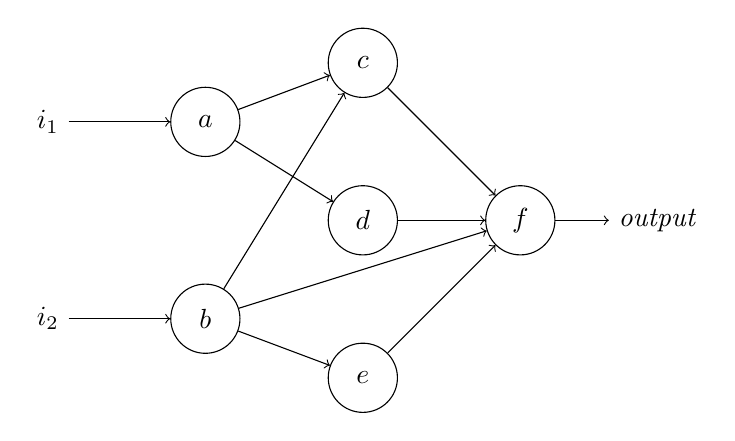
\begin{tikzpicture}
\node (i1)[] at (0, 3.25) {$i_1$};
\node (i2)[] at (0, 0.75) {$i_2$};
\node (a)[circle, draw, minimum width=25pt] at (2, 3.25) {$a$};
\node (b)[circle, draw, minimum width=25pt] at (2, 0.75) {$b$};
\node (c)[circle, draw, minimum width=25pt] at (4, 4) {$c$};
\node (d)[circle, draw, minimum width=25pt] at (4, 2) {$d$};
\node (e)[circle, draw, minimum width=25pt] at (4, 0) {$e$};
\node (f)[circle, draw, minimum width=25pt] at (6, 2) {$f$};
\node (output)[] at (7.75, 2) {$\mathit{output}$};
\draw[->] (i1) -- (a) ;
\draw[->] (i2) -- (b) ;
\draw[->] (a) -- (c);
\draw[->] (a) -- (d);
% \draw[->] (a) -- (e);
\draw[->] (b) -- (c);
\draw[->] (b) -- (f);
\draw[->] (b) -- (e);
\draw[->] (c) -- (f);
\draw[->] (d) -- (f);
\draw[->] (e) -- (f);
\draw[->] (f) -- (output);
\end{tikzpicture}
\end{minipage}~\\[2.5pt]
\scalebox{0.7}{
\begin{tikzpicture}
\node[draw,minimum width=0.5cm, minimum height=0.5cm] at (0,0) {0};
\node[draw,minimum width=0.5cm, minimum height=0.5cm] at (0.5,0) {0};
\node[draw,minimum width=0.5cm, minimum height=0.5cm] at (1,0) {0};
\node[draw,minimum width=0.5cm, minimum height=0.5cm] at (1.5,0) {0};
\node[draw,minimum width=0.5cm, minimum height=0.5cm] at (2,0) {0};
\node[draw,minimum width=0.5cm, minimum height=0.5cm] at (2.5,0) {0};
\node[draw,minimum width=0.5cm, minimum height=0.5cm] at (3,0) {0};
\node[draw,minimum width=0.5cm, minimum height=0.5cm] at (3.5,0) {0};
\node[draw,minimum width=0.5cm, minimum height=0.5cm] at (4,0) {0};
\node[draw,minimum width=0.5cm, minimum height=0.5cm] at (4.5,0) {0};
\node[draw,minimum width=0.5cm, minimum height=0.5cm] at (5,0) {0};
\node[draw,minimum width=0.5cm, minimum height=0.5cm] at (5.5,0) {0};
\node[draw,minimum width=0.5cm, minimum height=0.5cm,fill=hured!20] at (6,0) {1};
\node[draw,minimum width=0.5cm, minimum height=0.5cm,fill=hured!20] at (6.5,0) {1};
\node[draw,minimum width=0.5cm, minimum height=0.5cm] at (7,0) {0};
\node[draw,minimum width=0.5cm, minimum height=0.5cm] at (7.5,0) {0};
\node[draw,minimum width=0.5cm, minimum height=0.5cm] at (8,0) {0};
\node[draw,minimum width=0.5cm, minimum height=0.5cm] at (8.5,0) {0};
\node[draw,minimum width=0.5cm, minimum height=0.5cm,fill=hured!20] at (9,0) {1};
\node[draw,minimum width=0.5cm, minimum height=0.5cm] at (9.5,0) {0};
\node[draw,minimum width=0.5cm, minimum height=0.5cm] at (10,0) {0};
\node[draw,minimum width=0.5cm, minimum height=0.5cm] at (10.5,0) {0};
\node[draw,minimum width=0.5cm, minimum height=0.5cm] at (11,0) {0};
\node[draw,minimum width=0.5cm, minimum height=0.5cm] at (11.5,0) {0};
\node[draw,minimum width=0.5cm, minimum height=0.5cm] at (12,0) {0};
\node[draw,minimum width=0.5cm, minimum height=0.5cm,fill=hured!20] at (12.5,0) {1};
\node[draw,minimum width=0.5cm, minimum height=0.5cm] at (13,0) {0};
\node[draw,minimum width=0.5cm, minimum height=0.5cm] at (13.5,0) {0};
\node[draw,minimum width=0.5cm, minimum height=0.5cm] at (14,0) {0};
\node[draw,minimum width=0.5cm, minimum height=0.5cm] at (14.5,0) {0};
\node[draw,minimum width=0.5cm, minimum height=0.5cm] at (15,0) {0};
\node[draw,minimum width=0.5cm, minimum height=0.5cm,fill=hured!20] at (15.5,0) {1};
\node[draw,minimum width=0.5cm, minimum height=0.5cm,fill=hured!20] at (16,0) {1};
\node[draw,minimum width=0.5cm, minimum height=0.5cm,fill=hured!20] at (16.5,0) {1};
\node[draw,minimum width=0.5cm, minimum height=0.5cm,fill=hured!20] at (17,0) {1};
\node[draw,minimum width=0.5cm, minimum height=0.5cm] at (17.5,0) {0};
\node at (1,1) {Chromosome:};
\draw[ultra thick] (-0.25,-0.25) rectangle (2.75,0.25);
\draw[ultra thick] (2.75,-0.25) rectangle (5.75,0.25);
\draw[ultra thick] (5.75,-0.25) rectangle (8.75,0.25);
\draw[ultra thick] (8.75,-0.25) rectangle (11.75,0.25);
\draw[ultra thick] (11.75,-0.25) rectangle (14.75,0.25);
\draw[ultra thick] (14.75,-0.25) rectangle (17.75,0.25);
\draw[decorate,decoration={brace,amplitude=10pt}] (2.75,-0.5) -- (-0.25, -0.5);
\node at (1.25, -1) {Gene};
\end{tikzpicture}}
\end{center}
We now apply our typical evolutionary components (fitness, selection, recombination, etc.) to obtain the following optimisation cycle:
\begin{center}
\newcommand\neuralnet[4]{
  \foreach \x in {0,...,36} {
    \draw (#1+\x*0.1, #2) rectangle (#1+0.1+\x*0.1,#2+0.25);
  }
  \foreach \x in {#3} {
    \draw[fill=hured!60] (#1+\x*0.1, #2) rectangle (#1+0.1+\x*0.1, #2+0.25);
  }
}
\begin{tikzpicture}
% \draw[step=1cm, gray, thin] (0,0) grid (12, 12);
% Current Generation genomes
\draw[fill=white] (4,12) rectangle (8,8);
\draw[fill=white] (4.1,11.9) rectangle (8.1,7.9);
\draw[fill=white] (4.2,11.8) rectangle (8.2,7.8);
% Top individual title
\node at (6.2, 11.5) {\textit{neural network}}; 
% Top individual genome
\neuralnet{4.35}{10.5}{12,13,18,25,26,32,33,34,35};
% Top individual neural net
\node (i1)[] at (4.55, 9.75) {\tiny $i_1$};
\node (i2)[] at (4.55, 9) {\tiny $i_2$};
\node (a)[circle, draw] at (5.35, 9.75) {\tiny $a$};
\node (b)[circle, draw] at (5.35, 9) {\tiny $b$};
\node (c)[circle, draw] at (6.5, 10) {\tiny $c$};
\node (d)[circle, draw] at (6.5, 9.25) {\tiny $d$};
\node (e)[circle, draw] at (6.5, 8.5) {\tiny $e$};
\node (f)[circle, draw] at (7.35, 9) {\tiny $f$};
\node (output)[] at (8.1, 9) {};
\draw[->] (i1) -- (a) ;
\draw[->] (i2) -- (b) ;
\draw[->] (a) -- (c);
\draw[->] (a) -- (d);
% \draw[->] (a) -- (e);
\draw[->] (b) -- (c);
\draw[->] (b) -- (f);
\draw[->] (b) -- (e);
\draw[->] (c) -- (f);
\draw[->] (d) -- (f);
\draw[->] (e) -- (f);
\draw[->] (f) -- (output);
\node at (6.2, 8.1) {\footnotesize\textit{fitness}$=117$};

\draw[fill=white] (-1,4) rectangle (3,8);
\node at (1, 7.75) {\textit{generation} $i$};
\neuralnet{-0.85}{7.25}{12,13,18,25,26,32,33,34,35};
\neuralnet{-0.85}{6.75}{12,18,24,25,30,31,32,33,34,35};
\neuralnet{-0.85}{6.25}{12,13,19,24,30,32,33,34};
\neuralnet{-0.85}{5.75}{12,18,25,32,35};
\neuralnet{-0.85}{5.25}{13,18,19,24,25,33,34,35};
\neuralnet{-0.85}{4.75}{12,19,24,30,31,34,35};
\neuralnet{-0.85}{4.25}{12,13,18,25,31,32,33,34,35};
\draw[fill=white] (0, 4.25) rectangle (4, 0.25);
\node at (2, 4) {\textit{generation} $i+1$};
\neuralnet{0.15}{3.5}{12,13,18,25,26,32,33,34,35};
\neuralnet{0.15}{3}{12,13,18,24,30,32,33,34,35};
\neuralnet{0.15}{2.5}{12,13,19,25,32,33,34};
\neuralnet{0.15}{2}{12,13,18,24,30,32,34,35};
\neuralnet{0.15}{1.5}{12,18,25,32,35};
\neuralnet{0.15}{1}{13,18,19,24,25,33,34,35};
\neuralnet{0.15}{0.5}{12,13,18,25,31,32,33,34,35};

\draw[fill=white] (9, 8) rectangle (13, 4.5);
\node at (11, 7.75) {\textit{crossover}};
\neuralnet{9.15}{7}{12,13,18,25,26,32,33,34,35};
\neuralnet{9.15}{6.25}{12,13,19,24,30,32,33,34};
\draw[fill=white,white] (11.55, 7.30) rectangle (12.25, 6.2);
  \draw[fill=white] (11.6, 7.1) rectangle (11.7, 7.35);
  \draw[fill=hured!60] (11.7, 7.1) rectangle (11.8, 7.35);
  \draw[fill=hured!60] (11.8, 7.1) rectangle (11.9, 7.35);
  \draw[fill=white] (11.9, 7.1) rectangle (12.0, 7.35);
  \draw[fill=white] (12.0, 7.1) rectangle (12.1, 7.35);
  \draw[fill=white] (12.1, 7.1) rectangle (12.2, 7.35);
  \draw[fill=white] (12.2, 7.1) rectangle (12.3, 7.35);
  \draw[fill=hured!60] (11.6, 6.35) rectangle (11.7, 6.6);
  \draw[fill=white] (11.7, 6.35) rectangle (11.8, 6.6);
  \draw[fill=white] (11.8, 6.35) rectangle (11.9, 6.6);
  \draw[fill=white] (11.9, 6.35) rectangle (12.0, 6.6);
  \draw[fill=white] (12.0, 6.35) rectangle (12.1, 6.6);
  \draw[fill=white] (12.1, 6.35) rectangle (12.2, 6.6);
  \draw[fill=hured!60] (12.2, 6.35) rectangle (12.3, 6.6);
  \draw[<->] (12, 7.05) to (12, 6.65);
\node[anchor=west] at (9.15, 5.85) {\textit{children:}};
\neuralnet{9.15}{5.25}{12,13,18,24,30,32,33,34,35};
\neuralnet{9.15}{4.75}{12,13,19,25,26,32,33,34};
\draw[fill=white] (9, 3) rectangle (13, 1);
\node at (11, 2.75) {\textit{mutation}};
\neuralnet{9.15}{2}{12,13,18,24,30,32,33,34,35};
\node at (12.5,2.1) {x};
\draw[->] (12.5, 1.9) to (12.5, 1.6);
\neuralnet{9.15}{1.25}{12,13,18,24,30,32,34,35};

\draw[fill=white] (4.5, 6.5) rectangle (8, 2.25);
\node at (6.25, 6.25) {\textit{training data set}};
\node at (6.25,4.1) {\scriptsize
$\begin{array}{rrr}
0&0&1.0000\\
0.1000&0.0998&0.8869\\
0.2000&0.1987&0.7551\\
0.3000&0.2955&0.6142\\
0.4000&0.3894&0.4720\\
0.5000&0.4794&0.3345\\
0.6000&0.5646&0.2060\\
0.7000&0.6442&0.0892\\
0.8000&0.7174&-0.0143\\
0.9000&0.7833&-0.1038\\
1.0000& 0.8415&-0.1794
\end{array}$
};

% Arrows $
\draw[blArrow] (11, 4.4) to (11, 3.1);
\draw[blArrow] (11, 0.9) -- (11, -0.75) -- (1.5, -0.75) to (1.5, 0.15);
\draw[blArrow] (1.5, 8.1) -- (1.5, 10) to (3.9, 10);
\draw[blArrow] (8.3, 10) -- (11, 10) to (11, 8.1);
\draw[blArrow] (6.25, 6.6) to (6.25, 7.7);
\node at (10, 10.5) {\textit{selection}};
\end{tikzpicture}
\end{center}

This method of encoding (called \textit{direct encoding}) and evolving the topology of neural networks becomes increasingly cumbersome when the complexity of the network rises (when more and more nodes are added). As the size of the network grows, the size of the required chromosome increases quickly, leading to problems in performance. Moreover, direct encoding cannot represent repeated or nested structures in the network, which are common for some problems.

An alternative encoding, called \textit{grammatical encoding} tries to solve this problem. This encoding represents the network encoding as grammars; the genetic algorithm evolves the grammars, but the fitness is tested only after a ``development'' step in which a network develops from the grammar. That is, the grammar is a ``genotype'', while the ``phenotype'' is a network derived from that grammar. The exact encoding scheme used in this method, and the execution of it are beyond the scope of this discussion.


\subsection{Evolving weights}
While this subject is beyond the scope of this course, as we have learned back-propagation in Section \ref{sec:gradient}. Back-propagation is in most situation the better way of learning the weights in a neural network, and is therefore preferred. In some situations, however, back-propagation can get stuck in one of the many local optima present, and has difficulties escaping these. In such cases, using a genetic algorithm to learn the weights instead could be helpful.

To apply genetic algorithms to the learning of weights, we use the vector representation as presented in the previous chapter. The chromosomes in our population are a sequence of (real) numbers, where each number represents a weight of a connection in the neural network. We group numbers related to a single neuron in a gene:
\begin{center}
\begin{tikzpicture}
\node (a)[circle, draw, minimum width=25pt] at (2, 1) {$a$};
\node (b)[circle, draw, minimum width=25pt] at (2, 0) {$b$};
\node (c)[circle, draw, minimum width=25pt] at (2, -1) {$c$};
\node (d)[circle, draw, minimum width=25pt] at (4, 1.5) {$d$};
\node (e)[circle, draw, minimum width=25pt] at (4, 0.5) {$e$};
\node (f)[circle, draw, minimum width=25pt] at (4, -0.5) {$f$};
\node (g)[circle, draw, minimum width=25pt] at (4, -1.5) {$g$};
\node (h)[circle, draw, minimum width=25pt] at (6, 0) {$h$};
\node (i1)[] at (0, 1) {$i_1$};
\node (i2)[] at (0, 0) {$i_2$};
\node (i3)[] at (0, -1) {$i_3$};
\node (output)[] at (7.75, 0) {$\mathit{output}$};
\draw[->] (i1) -- (a) ;
\draw[->] (i2) -- (b) ;
\draw[->] (i3) -- (c) ;
\draw[->,hured] (a) -- (d);
\draw[->] (a) -- (e);
\draw[->] (a) -- (f);
\draw[->] (a) -- (g);
\draw[->,hured] (b) -- (d);
\draw[->] (b) -- (e);
\draw[->] (b) -- (f);
\draw[->] (b) -- (g);
\draw[->,hured] (c) -- (d);
\draw[->] (c) -- (e);
\draw[->] (c) -- (f);
\draw[->] (c) -- (g);
\draw[->,hublue] (d) -- (h);
\draw[->,hublue] (e) -- (h);
\draw[->,hublue] (f) -- (h);
\draw[->,hublue] (g) -- (h);
\draw[->] (h) -- (output);

\node[anchor=south west] at (-2,-2.5) {Chromosome:};
\node[anchor=south west,draw,minimum height=1cm,minimum width=1cm,fill=hured!20] at (-2,-3.5) {\footnotesize $w_{a\rightarrow d}$};
\node[anchor=south west,draw,minimum height=1cm,minimum width=1cm,fill=hured!20] at (-1,-3.5) {\footnotesize $w_{b\rightarrow d}$};
\node[anchor=south west,draw,minimum height=1cm,minimum width=1cm,fill=hured!20] at (0,-3.5) {\footnotesize $w_{c\rightarrow d}$};
\node[anchor=south west,draw,minimum height=1cm,minimum width=1cm] at (1,-3.5) {\footnotesize $w_{a\rightarrow e}$};
\node[anchor=south west,draw,minimum height=1cm,minimum width=1cm] at (2,-3.5) {\footnotesize $w_{b\rightarrow e}$};
\node[anchor=south west,draw,minimum height=1cm,minimum width=1cm] at (3,-3.5) {\footnotesize $w_{c\rightarrow e}$};
\node[anchor=south west] at (4.15,-3.25) {\ldots};
\node[anchor=south west,draw,minimum height=1cm,minimum width=1cm] at (5,-3.5) {\footnotesize $w_{c\rightarrow g}$};
\node[anchor=south west,draw,minimum height=1cm,minimum width=1cm,fill=hublue!20] at (6,-3.5) {\footnotesize $w_{d\rightarrow h}$};
\node[anchor=south west,draw,minimum height=1cm,minimum width=1cm,fill=hublue!20] at (7,-3.5) {\footnotesize $w_{e\rightarrow h}$};
\node[anchor=south west,draw,minimum height=1cm,minimum width=1cm,fill=hublue!20] at (8,-3.5) {\footnotesize $w_{f\rightarrow h}$};
\node[anchor=south west,draw,minimum height=1cm,minimum width=1cm,fill=hublue!20] at (9,-3.5) {\footnotesize $w_{g\rightarrow h}$};
\draw[decorate,decoration={brace,amplitude=10pt}] (1, -3.75) -- (-2, -3.75);
\node at (-0.5, -4.5) {Gene};
\end{tikzpicture}
\end{center}

Next we need to define a fitness function for evaluating the performance of the chromosomes. The function must estimate the performance of a given network, which can easily be calculated by having the network classify a number of examples. The number of examples should not be too small, since this increases the risk of overfitting (the neural network performs well on the examples, but not on the real problem). However, too much examples means that the evaluation of a population takes more time. An alternative is to select a portion of a large data set for testing every selection round (but make sure that all networks are scored using the same examples).

The simplest function to score networks (based on an example set) is using the sum of squared errors (see Section \ref{sec:gradient} earlier for details). The smaller the sum, the fitter the network. This means that the genetic algorithm attempts to find a set of weights that minimises the sum of squared errors.

There are a number of choices for the genetic operators. In some cases, an evolutionary strategy is used which means that only mutation is allowed, but crossover can be applied as well, if designed correctly. A crossover operator (single-point crossover, two-point crossover, or even uniform crossover) needs to adhere to the weights that belong to a single neuron; that is, crossover can be performed, as long as the crossover points are chosen to match the gene encoding, that is, split only on the segments that represent the weights on the links related to a single neuron.
\begin{center}
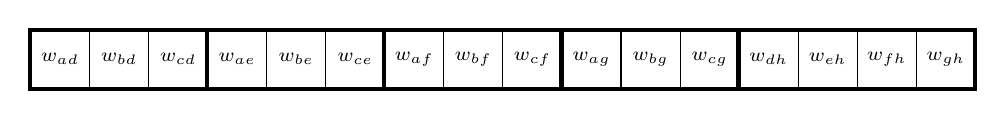
\begin{tikzpicture}[font=\scriptsize]
\node[anchor=south west,thin,draw,minimum width=0.75cm,minimum height=0.75cm] at (0,   0) {$w_{ad}$};
\node[anchor=south west,thin,draw,minimum width=0.75cm,minimum height=0.75cm] at (0.75,0) {$w_{bd}$};
\node[anchor=south west,thin,draw,minimum width=0.75cm,minimum height=0.75cm] at (1.5, 0) {$w_{cd}$};
\node[anchor=south west,thin,draw,minimum width=0.75cm,minimum height=0.75cm] at (2.25,0) {$w_{ae}$};
\node[anchor=south west,thin,draw,minimum width=0.75cm,minimum height=0.75cm] at (3,   0) {$w_{be}$};
\node[anchor=south west,thin,draw,minimum width=0.75cm,minimum height=0.75cm] at (3.75,0) {$w_{ce}$};
\node[anchor=south west,thin,draw,minimum width=0.75cm,minimum height=0.75cm] at (4.5, 0) {$w_{af}$};
\node[anchor=south west,thin,draw,minimum width=0.75cm,minimum height=0.75cm] at (5.25,0) {$w_{bf}$};
\node[anchor=south west,thin,draw,minimum width=0.75cm,minimum height=0.75cm] at (6,   0) {$w_{cf}$};
\node[anchor=south west,thin,draw,minimum width=0.75cm,minimum height=0.75cm] at (6.75,0) {$w_{ag}$};
\node[anchor=south west,thin,draw,minimum width=0.75cm,minimum height=0.75cm] at (7.5, 0) {$w_{bg}$};
\node[anchor=south west,thin,draw,minimum width=0.75cm,minimum height=0.75cm] at (8.25,0) {$w_{cg}$};
\node[anchor=south west,thin,draw,minimum width=0.75cm,minimum height=0.75cm] at (9,   0) {$w_{dh}$};
\node[anchor=south west,thin,draw,minimum width=0.75cm,minimum height=0.75cm] at (9.75,0) {$w_{eh}$};
\node[anchor=south west,thin,draw,minimum width=0.75cm,minimum height=0.75cm] at (10.5,0) {$w_{fh}$};
\node[anchor=south west,thin,draw,minimum width=0.75cm,minimum height=0.75cm] at (11.25,0) {$w_{gh}$};
\draw[ultra thick] (0,0) rectangle (2.25,0.75);
\draw[ultra thick] (2.25,0) rectangle (4.5,0.75);
\draw[ultra thick] (4.5,0) rectangle (6.75,0.75);
\draw[ultra thick] (6.75,0) rectangle (9,0.75);
\draw[ultra thick] (9,0) rectangle (12, 0.75);
% \draw[ultra thick] (2.25, 1.25) -- (2.25, -0.5)
%                    (4.5,  1.25) -- (4.5,  -0.5)
%                    (6.75, 1.25) -- (6.75, -0.5)
%                    (9,    1.25) -- (9,    -0.5);
\end{tikzpicture}
\end{center}

The mutation operator can be chosen, for instance, to add a small random value between $-1$ and $1$ to each weight in a randomly chosen gene (again, remember that a single gene represents multiple weights).

As mentioned at the start of this section, while the optimisation of weights of a neural network by means of an evolutionary algorithm is possible, it is rarely used. This is because the genetic algorithm has many more parameters that need to be selected to find the optimal training strategy, and because back-propagation usually functions well enough. The latter is especially true in larger (thousands to millions of neurons) networks.

\section{Exercises}
%Choose and solve either exercise \ref{ex:card} or \ref{ex:wing}; they are different flavours of the same kind of problem:
\begin{exercise}[Card problem]\label{ex:card}~\\
You have 10 cards numbered from 1 to 10. You have to choose a way of dividing them into two piles, so that the cards in the first pile \textbf{sum} to a number as close as possible to 36, and the remaining cards in the other pile \textbf{multiply} to a number as close as possible to 360.

\paragraph{Genotype encoding}
Each card can be put in \pythoninline{Pile_0} or \pythoninline{Pile_1}, there are 1024 possible ways of sorting them into two piles, and you have to find the best. Think of a sensible way of encoding any possible solution-attempt as a genotype.

\paragraph{Fitness}
Some of these solution attempts will be closer to the target than others. Think of a sensible way of evaluating any solution-attempt and scoring it with a fitness-measure.

\paragraph{Assignment}
Write a program to run a Genetic Algorithm with your genotype encoding and fitness function.
Run it once for a suitable (probably very large -- you choose) number of generations.
Then repeat that same run a number of times (like, 100) and see if you get the same answer each time, see how much variance there is between each run.
\end{exercise}

\begin{exercise}[Wing design]\label{ex:wing}~\\
You have 4 variables that represent possible parameter settings for the design of an aircraft wing. $A$, $B$, $C$, and $D$, each of which can be any whole number between 0 and 63 (use a bit encoding per parameter).

\noindent Your aerodynamics model tells you that the $\mathit{Lift}$ of the wing is the following:
$$\mathit{Lift} = (A-B)^2+(C+D)^2-(A-30)^3-(C-40)^3$$

\noindent Find values of $A$ $B$ $C$ $D$, each within their allowed range 0-63, that maximises $\mathit{Lift}$.

\paragraph{Assignment}
Write a program to run a Genetic Algorithm with your genotype encoding and fitness function.
Run it once for a suitable (probably very large -- you choose) number of generations.
Then repeat that same run a number of times (like, 100) and see if you get the same answer each time, see how much variance there is between each run.
\end{exercise}

\begin{exercise}[Face Recognition (Optional)]~\\
In this exercise we are going to combine evolutionary algorithms with neural networks to create a facial recognition system.

A data set consisting of pictures (96$\times$96 pixels, greyscale) is available on the electronic learning environment. The images are pictures (centered) of lecturers of the Computer Engineering team. Your task is to use the available data set to create and train a neural network that can detect which person is represented on a given image.

Use an evolutionary algorithm to determine the most suitable configuration (topology, etc.) of your neural network. The neural networks should be created by using available library implementation\footnote{For example, see Appendix \ref{ch:lib} for descriptions of the use of neural network libraries, including \pythoninline{TensorFlow} and \pythoninline{Theano}. You are not restricted to either of these, you may choose your own.}

The optimisation of the network and the training of the neural network are done in \textit{your} time; during grading we will assess how well your (best) neural network performs on a new set of images. That means that you need to be able to save (and later load) a neural network (layers, weights, etc.).

\paragraph{Hand-in}
You need to hand-in the following elements:
\begin{itemize}
\item the implementation (code) of the evolutionary algorithm that was used to determine the NN architecture;
\item a short description of the best architecture (found by your EA) (describe number of layers, layer types, etc.) and a brief explanation why you think this is the best architecture;
\item an implementation (code) that can read your best network and perform a classification based on a given (similar, but different) dataset to assess it's performance.
\end{itemize}
\end{exercise}
